\RequirePackage{plautopatch}

% \documentclass[dvipdfmx]{jsbook}
\documentclass[uplatex,dvipdfmx]{jsbook}
% \documentclass{ltjsbook}

\usepackage{graphicx}
\usepackage[top=20truemm,bottom=20truemm,left=30truemm,right=20truemm]{geometry}
\usepackage{amsmath, amssymb}
\usepackage{fancybox}
\usepackage{here}
\usepackage{eclbkbox}
\usepackage{tcolorbox}
\usepackage[hidelinks]{hyperref}
\usepackage{url}
\usepackage[T1]{fontenc}

\newcommand{\nendo}{2023}
\newcommand{\hann}{\nendo 年度版}

\newcommand{\til}{\char`\~}
\newcommand{\promptn}{\$}
\newcommand{\prompt}{\$ }
\newcommand{\pager}{\textbf{less}}
\newcommand{\ctrl}[1]{\ovalbox{\mathstrut ctrl}-\ovalbox{\mathstrut #1}}
\newcommand{\esc}[1]{\leavevmode\ovalbox{\mathstrut Esc}-\ovalbox{\mathstrut #1}}
\newcommand{\ret}{\ovalbox{\mathstrut Enter}}
\newcommand{\spc}{\leavevmode\ovalbox{\mathstrut スペース}}
\newcommand{\BS}{\ovalbox{\mathstrut Backspace}\ あるいは \ovalbox{\mathstrut Delete}キー}
\newcommand{\cursor}{\vrule height8pt depth3pt width4pt\relax}
\newcommand{\itemf}[1]{\item \textbf{#1}}

\newsavebox{\fminibox}
\newenvironment{myframe}[2][\textwidth]%
{\vspace{12pt}\newline\begin{minipage}{#1}\textbf{#2}\newline%
    \begin{lrbox}{\fminibox}\begin{minipage}{#1}}%
{\end{minipage}\end{lrbox}\fbox{\usebox{\fminibox}}\end{minipage}\vspace{12pt}}

\newenvironment{myframe2}[1]{%
  \vspace{12pt}%
  \begin{breakbox}%
  {\parindent=0pt\textbf{\underline{#1}}}%
}{%
  \end{breakbox}\vspace{12pt}%
}

\newenvironment{myframe3}[1]{%
  \vspace{12pt}%
  {\parindent=0pt\textbf{\underline{#1}}}\quad%
}{%
  \vspace{12pt}
}

%%% 例環境
\newcounter{reidai}[section]
\def\thereidai{\thesection.\arabic{reidai}.}
\newenvironment{reidai}{%
  \refstepcounter{reidai}%
  \begin{myframe2}{例 \thereidai}%
  \baselineskip=12pt%
  \begin{quote}%
}{%
  \end{quote}%
  \end{myframe2}%
}

\newcounter{kekka}[section]
\def\thekekka{\thereidai}
\newenvironment{kekka}%
{\refstepcounter{kekka}
  \begin{myframe2}{結果 \thekekka}
  \baselineskip=12pt%
  \begin{quote}%
}{%
  \end{quote}%
  \end{myframe2}%
}


%%% 練習環境
\newenvironment{commandline2}{%
  %\begin{quote}
  \begin{tcolorbox}\tt%
}{%
  \end{tcolorbox}%
  %\end{quote}%
}

\newcounter{renshuu}[section]
\def\therenshuu{\thesection.\arabic{renshuu}.}
\newenvironment{renshuu}{%
  \refstepcounter{renshuu}%
  \begin{myframe3}{練習 \therenshuu}%
}{%
  \end{myframe3}%
}

\newenvironment{renshuu-answer}[1]{%
  \begin{myframe2}{練習 \ref{#1}}
  \begin{quote}%
}{%
  \end{quote}%
  \end{myframe2}%
}

\newcommand{\esckey}{\texttt{\ovalbox{Esc}}}
\newcommand{\tabkey}{\texttt{\ovalbox{Tab}}}
\newcommand{\typecom}[2][\ret]{\begin{quote}{\tt\prompt \underline{#2} }#1\end{quote}}
\newcommand{\typeans}[1]{\begin{quote}\tt#1 \end{quote}}

\def\clangpara#1{\paragraph{#1}\mbox{}\\}

\newenvironment{commandline}%
{\vspace{6pt}\newline\hspace{26pt}\begin{minipage}{\textwidth}}%
{\end{minipage}\vspace{6pt}}

\makeatletter
\@addtoreset{equation}{section}
\makeatother

% \def\labelitemi{$\Rightarrow$}

\pagestyle{plain}

\begin{document}
\thispagestyle{empty}
\pagestyle{empty}
\begin{titlepage}
    \vspace*{5cm}
    \begin{center}
        \textbf{\Huge 計算機実験ハンドブック}\\
        \vspace*{14cm}
        \textbf{\LARGE \hann}\\
        \vspace{1.0cm}
        \textbf{\LARGE 東京大学理学部物理学科}
    \end{center}
\end{titlepage}
\clearpage
\pagestyle{empty}
\cleardoublepage

\section*{はじめに}

\noindent
理学部物理学科3年の講義「計算機実験I」および「計算機実験II」は、理論・実験を問わず、学部〜大学院〜で必要とされる現代的かつ普遍的な計算機の素養を身につけることを目標としている。基礎的な数値計算アルゴリズムとその応用を学習するだけでなく、実習を通じて、計算機の操作、C言語を用いたプログラミング技術、\LaTeX による科学論文の作成技術などを学ぶ。
本冊子は、「計算機実験I」および「計算機実験II」の時間に、より効果的に実習を進めることができるよう、必要とされる技術的な点をまとめたものである。
なお、実習に必要となる環境の準備については、「計算機実習のための環境整備」(\url{https://utphys-comp.github.io})にまとめてあるので、そちらを参照してほしい。
また、教育用計算機システムECCSの端末を用いる場合は、\url{https://www.ecc.u-tokyo.ac.jp/} にある情報を参照のこと。

\clearpage
\section*{改訂履歴}

\noindent
\begin{description}
\item[2019年度版 (2019年9月)] \mbox{}
  
  \begin{itemize}
  \item SSHの公開鍵認証についての記述を追加
  \item Gnuplotのファイルへの出力、\LaTeX への図の取り込みをEPS形式からPDF形式に変更
  \item 動的な二次元配列についての記述を追加
  \end{itemize}

\item[2018年度版 (2018年9月)] \mbox{}
  
  \begin{itemize}
  \item Gnuplotについての解説を充実
  \item バージョン管理システムの章を別ファイルに
  \end{itemize}

\item[2017年度版 (2017年4月)] \mbox{}
  
  \begin{itemize}
  \item 名称を「計算機実験ハンドブック」に変更
  \item バージョン管理システムの中のURLを修正
  \end{itemize}

\item[2016年度版 (2016年4月)] \mbox{}

  \begin{itemize}
  \item ECCS2016にあわせて改訂
  \end{itemize}

\item[2015年度版 (2015年4月)] \mbox{}

  \begin{itemize}
  \item 改訂新版
  \item 付録にバージョン管理システムを追加
  \end{itemize}

\end{description}

\cleardoublepage

\setcounter{page}{1}
\setcounter{tocdepth}{3}
\tableofcontents

\clearpage
\pagestyle{plain}
\cleardoublepage

\chapter{UNIX入門}

\noindent
この章では、UNIXと呼ばれるOS (オペレーティングシステム)の操作法について学ぶ。通常、macOSやWindowsでは、マウスを使って画面を操作する。実は、macOSの内部ではDarwinと呼ばれるUNIX系のOSが動作しており、「ターミナル」アプリケーションを立ち上げることにより、UNIXの様々な機能に直接アクセスすることができる。また、ワークステーションやスーパーコンピュータなど、より大きな規模の計算を行うことのできる計算機も、ほぼ全てLinuxなどのUNIX系OSである。
UNIX系のOSの特徴としては、シンプル、柔軟かつオープンであり、ネットワークに強いことが挙げられる。シェルやスクリプト言語を組み合わせることにより、簡単なコマンドで複雑な処理を実現することができる。また、ネットワーク経由で使用することが前提となっており、実際に計算機がどこにあるかを意識することなしに、透過的に利用できる。UNIXを取得することにより、目の前のPCだけでなく世界中の計算機を利用することが可能となり、計算能力が一気に増えることになる。

\section{UNIX のコマンド}

この節での操作はすべて、ターミナル(「シェル」とも呼ぶ)内でコマンドを打ち込み、最後にリターンキーを押すことより実行する。下線を引いた部分がキーボードからの入力である。行頭の``\texttt {\promptn}''はプロンプトと呼ばれる。UNIXのシェルがユーザからのコマンド入力待ちの状態であることを示すものであり、コマンド入力時にタイプする必要はない。

\subsection{ファイルの操作}
\label{sec:unix:fileManagement}
この節では、ファイルを作ったり、消したりといった基本的な操作を紹介する。ファイルというのは計算機が情報を書き込むための一つの単位である。ファイルには名前を付けることができて、その名前を指定することでファイルを編集したり消したりできる。

\subsubsection*{ファイルの基本操作}
ファイルをコピーするには{\tt cp}コマンド({\bf c}o{\bf p}yの略)を用いる。例えば、コマンドラインで
\begin{commandline2}
\prompt \underline{cp /usr/local/example/circle.c circle.c}
\end{commandline2} \noindent
を実行すると、{\tt /usr/local/example}という名前のディレクトリにあるファイル{\tt circle.c}が、カレントディレクトリにコピーされる。{\tt /usr/local/example/circle.c}の部分がコピー元に対応し、後の{\tt circle.c}がコピー先を意味する。コピー先がディレクトリの場合には、コピー先のディレクトリにコピー元と同じ名前のファイルが作られる。したがって、上の例は、カレントディレクトリを表す ``{\tt .}'' を用いて、
\begin{commandline2}
\prompt \underline{cp /usr/local/example/circle.c .}
\end{commandline2} \noindent
としても同じ結果となる。元とは異なる名前でコピーしたい場合には、
\begin{commandline2}
\prompt \underline{cp /usr/local/example/circle.c oval.c}
\end{commandline2} \noindent
などとする。同じ名前のファイルがすでに存在する場合には上書きされるので注意せよ。

ここで、{\tt ls}コマンド({\bf l}i{\bf s}tの略)を実行すると
\begin{commandline2}
\prompt \underline{ls}
\vspace*{-.8em} 
\begin{verbatim}
Desktop    circle.c
\end{verbatim}
\end{commandline2} \noindent
と表示され、正しくコピーされたことが分かる。このように、{\tt ls}コマンドを使うことで、どのようなファイルがあるのかを知ることができる。さらに、{\tt ls -l}を実行すると
\begin{commandline2}
\prompt \underline{ls -l}
\vspace*{-.8em} 
\begin{verbatim}
total 2
drwxr-xr-x  2 s001500 student      512 Apr 16 03:40 Desktop
-rw-r--r--  1 s001500 student      372 Apr 16 03:43 circle.c
\end{verbatim}
\end{commandline2} \noindent
のように、より詳細な情報\footnote{表示の1行目は、左端の {\tt d} が、そのファイルがディレクトリであることを示し、次の{\tt rwx}はファイルの所有者が読み取り可能({\tt r})、書き込み可能({\tt w})、実行可能({\tt x})であることを示している。(ディレクトリが読み取り可能であるとは、そのディレクトリにどのようなファイルが入っているかを{\bf ls}コマンドで調べられることをいい、ディレクトリが書き込み可能とは、そのディレクトリに新しくファイルやディレクトリを新しく作ったり、すでにあるファイルなどを消したりできることをいう。さらに、ディレクトリが実行可能であるとは、そのディレクトリ内部のファイルを操作できたり、そのディレクトリに移動するとか、そのディレクトリの名前をパスに含めることができることを意味する。) 次の{\tt r-x}は同じグループに所属する人が、読み取りと実行可能であることを示し、その次の{\tt r-x}はそのほかすべての人が読み取りと実行可能であることを示している。隣のカラムの{\tt s001500}は、そのファイルの所有者が{\tt s001500}であることを示し、次のカラムは所有グループを示している。次の{\tt 512}は、そのファイルの大きさが512 byteであることを示している。{\tt Apr 16 03:40}は、そのファイルに最後に変更を加えた日時を示す。そして最後がファイルの名前である。}を得ることができる。この{\tt -l}をオプション(あるいはコマンドラインオプション)と呼ぶ。{\tt ls}コマンドには他にも様々なオプションが用意されている。{\tt -F} オプションをつければ、ファイルの名前の後にファイルの種別を表す文字をつけてくれる。ディレクトリには {\tt /} が、実行可能ファイルには{\tt $ \ast$} がつく。{\tt -R} オプションをつければ、カレントディレクトリ以下のすべてのディレクトリの中身を見ることができる。また、{\tt -a} とすると、通常表示されない . (ピリオド)から始まるファイルも見ることができるようになる。

次にファイルの名前を変えてみよう。先の{\tt circle.c}を{\tt ring.c}に名前を変更するには、{\tt mv}コマンド({\bf m}o{\bf v}eの略)を使う。
\begin{commandline2}
\prompt \underline{mv circle.c ring.c}
\end{commandline2} \noindent
{\tt ls}コマンドで実際に名前が変更されたか確かめてみよう。

続いて{\tt rm}コマンド({\bf r}e{\bf m}oveの略)を用いてファイルを消してみよう。
\begin{commandline2}
\prompt \underline{rm ring.c}
\end{commandline2} \noindent
{\bf 一度消したファイルは二度と復旧できない}ので慎重に実行しなければならない。自信がないなら、
\begin{commandline2}
\prompt \underline{rm -i ring.c}
\end{commandline2} \noindent
のように{\tt -i}オプションをつけるとよい。ファイルごとに消してよいかどうかの確認をしてくれるので安心である。

さて、ここまでディレクトリという言葉が何度か出てきた。UNIXでは、ディレクトリという特殊なファイルを使って、たくさんのファイルをtree状に管理することができる。ディレクトリとは書類をまとめる書類箱だと思えばよいだろう。ときに大きな書類箱のなかに小さな書類箱が入っていることもあるわけで、ディレクトリの中にディレクトリがあってもいっこうに構わない。

ログインして最初にいるディレクトリのことをホームディレクトリと呼ぶ。今いるディレクトリ\footnote{カレントディレクトリ、あるいはワーキングディレクトリと呼ぶ。}がどこかを知るには、{\tt pwd}コマンド({\bf p}rint {\bf w}orking {\bf d}irectoryの略)を使う。{\tt /home/s001500} と表示されれば ルートディレクトリ\footnote{ルートディレクトリとは一番上のディレクトリのことであり、最初の{\tt /}がルートディレクトリを表す。}の下の {\tt home} というディレクトリの下の、{\tt s001500}というディレクトリにいるということが分かる。

試しに{\tt sample}という ディレクトリを作ってみよう\footnote{すでにあるディレクトリを消すには{\tt rmdir}コマンド({\bf r}e{\bf m}ove {\bf dir}ectoryの略)を使う。{\tt rmdir} でディレクトリを消すときはそのディレクトリの中にファイルやディレクトリが一つもない状態になっていなくてはならない。消したいディレクトリの中にファイルが残っているときは {\tt rm} コマンドを使い、ディレクトリが残っているときは {\tt rmdir} コマンドを使う。残っているファイルやディレクトリをいちいち消すのが面倒な場合は{\tt rm -r {\it directory}}とすれば、{\it directory}の中に何が残っていてもすべてきれいに消し去ってくれる。}。
\begin{commandline2}
\prompt \underline{mkdir sample}
\end{commandline2} \noindent
これで{\tt sample}というディレクトリが作成された。{\tt ls}コマンドで確かめてみよう。次に、今作ったディレクトリに移動してみよう。
\begin{commandline2}
\prompt \underline{cd sample}
\end{commandline2} \noindent
{\tt cd}は{\bf c}hange {\bf d}irectoryの略である。ここで、先ほどの {\tt cp}コマンドを使えば、このディレクトリにファイルをコピーすることができる。さらにこの中で \underline{{\tt mkdir chap4}} と打てば、{\tt sample}ディレクトリの下に{\tt chap4}ディレクトリが作成される。

では、元のディレクトリに戻るにはどうすればよいのだろうか? それには
\begin{commandline2}
\prompt \underline{cd ..}
\end{commandline2} \noindent
を実行する。{\tt cd}と{\tt ..}の間に空白があることに注意すること。

ツリー構造の中で、どのようにディレクトリやファイルを指定すればよいのだろうか。ディレクトリのツリーを図示すれば次のようになる。

\unitlength 1mm
\begin{picture}(100,85)(-30,-75)
\put(50,0){\fbox{/}}
\put(50,-5){\line(-2,-1){23}}\put(50,-5){\line(0,-1){13}}\put(50,-5){\line(2,-1){23}}
\put(25,-20){\fbox{home}}\put(47,-20){\fbox{usr}}\put(70,-20){\fbox{etc}}
\put(30,-24){\line(-2,-1){23}}\put(30,-24){\line(0,-1){12}}\put(30,-24){\line(2,-1){23}}
\put(0,-40){\fbox{hirano}}\put(25,-40){\fbox{s001500}  ...  }\put(50,-40){\fbox{s815xx} ....}
\put(28,-43){\line(-2,-1){23}}\put(28,-43){\line(0,-1){10}}\put(28,-43){\line(2,-1){23}}
\put(0,-56){\fbox{ftp}}\put(25,-55){\fbox{sample}}\put(50,-55){\fbox{tmp} ... }
\put(28,-58){\line(-2,-1){23}}\put(28,-58){\line(0,-1){10}}
\put(0,-72){\fbox{chap4}}\put(25,-72){\fbox{chap5} ... }
\end{picture}

\noindent このツリーの中の位置は、一番上の {\tt /} で表されるルートディレクトリから順にたどることより指定することができる。これを「絶対パス」と呼ぶ。あるいは、今いるディレクトリ(カレントディレクトリ)からの相対的な位置で指定する方法もある。これを「相対パス」と呼ぶ。例えば、ホームディレクトリの下の{\tt sample}の下の{\tt chap4}ディレクトリは、絶対的な指定では
\begin{tt}
/home/s001500/sample/chap4
\end{tt}
と書かれるが、カレントディレクトリがホームディレクトリの場合、相対的な指定では{\tt sample/chap4}と書かれる。そのディレクトリの中にあるファイルも {\tt /home/s001500/sample/chap4/circle.c}とか{\tt sample/chap4/circle.c}のように指定することができる。特に一つ上のディレクトリは``{\tt ..}''で、カレントディレクトリは``{\tt .}''であらわされる。つまり先ほどの{\tt sample/chap4/circle.c}は{\tt ./../s001500/sample/chap4/circle.c}と書いても同じものを指す。

これで、自由にディレクトリ間を移動することができるようになった。例えば、すでに使った{\tt ls}コマンドは、{\tt /usr/bin}あるいは{\tt /bin}ディレクトリに格納されている\footnote{\underline{\tt which ls}とすることで、{\tt ls}がどこにあるか調べることができる。}。\underline{\tt cd /usr/bin} として、そこに移動してから\underline{\tt ls}と打ってみよう。たくさんのファイルが置かれているが、{\tt ls} というファイルは見付かっただろうか\footnote{例えば、{\tt treasure.here}という名前のファイルを探したい場合、そのファイルがありそうなディレクトリよりも上のディレクトリに行って、\underline{\tt find . -name treasure.here -print}とする。{\tt find}の直後の {\tt .} (ピリオド)は「そのファイルがありそうなディレクトリより上のディレクトリのパス」を指定する。またファイル名があやふやな場合でも、\underline{\tt find . -name 'tre$\ast$.here' -print}のように$\ast$を任意の文字列として合致するファイルを表示してくれる。{\tt find}はとても多機能である。例えば\underline{\tt find . -name 'tre$\ast$.here' -exec cat \{\} $\backslash$;}のように、探し出したファイルに対してコマンドを実行することもできる。{\tt -exec} 以下の書式は コマンドの引数となるファイル名が\{\}となるように書き、最後に {\tt $\backslash$;} を加えればよい。{\tt -exec} の代わりに {\tt -ok} を使えばコマンドを実行する前に一々聞いて来るので {\tt rm}などを {\tt find} で実行したいときには安心である。\underline{\tt find\ .\ -ctime -1 -print}のように{\tt -ctime}で最終変更期日が1日前以内のものだけ表示させるようなことも可能である。{\tt -ctime}の引数を{\tt +1} にすると最終変更期日が1日以上前のものだけが表示される。}。

なお、\underline{{\tt cd}}とだけ打てば、いつでも自分のホームディレクトリに戻ってくることができる。ホームディレクトリは $\tilde{\ }$ とも表されるので \underline{{\tt cd $\tilde{\ }$}}としても同じである。

\subsubsection*{ファイルの中を見る}

さて、肝心のファイルの中身を見るにはどうしたらよいのだろう。ファイルの中身を見るにはいくつかの方法がある。ファイルには大別して、中身を見ることができるテキストファイルと中身を見られないバイナリファイルがある。テキストファイルの中身は、{\tt cat}コマンドで見ることができる\footnote{バイナリのファイルの中身を覗くための{\tt od} ({\bf o}ctal {\bf d}ump)というコマンドもある。}。
\begin{commandline2}
\prompt \underline{cat circle.c}
\end{commandline2} \noindent
{\tt cat}は最も手軽にファイルの中身をのぞくことのできるコマンドである。中身が長すぎる場合、{\tt cat}では流れていってしまうが、
\begin{commandline2}
\prompt \underline{more circle.c}
\end{commandline2} \noindent
と打つことにより、ちょうどよい所で一旦止めてくれる。\fbox{\tt --More--(xx\%)} のような表示が左下に見えたら、\spc を叩いてみよう。次のページが表示されるはずである。\underline{\tt h}と打つと簡単なヘルプが見られる。\underline{\tt b}か\ctrl{B}で1ページ戻る。また\ret で1行進む。さらに、\underline{\tt /}の後に\underline{\tt 文字列}を打つことでファイル中の文字列を検索することができる。検索された文字列を含む行はウインドウの一番上に表示される。\underline{\tt n}と打てばもう一度同じ文字列を探してくれる。また、\underline{\tt 10d}のように数字を入れてから\underline{\tt d}を打てば、その数字分だけ進む。{\tt more}から抜けるには、\underline{\tt q}を入力する。

{\tt more}と似ているが、もう少し使い勝手のよい{\tt less}\label{sect:less}というコマンドもある。{\tt less}では上向きにスクロールすることができる。\underline{\tt j}で1行下に、\underline{\tt k}で1行上\footnote{UNIX標準エディター {\tt vi} のキー操作と同じ。}に進む。{\tt more}と同じく、スペースバー、\underline{\tt h}、\underline{\tt b}、\underline{\tt d}、\underline{\tt /}、\underline{\tt n}、\underline{\tt q}のようなコマンドも使える。更に \underline{\tt g}でファイルの先頭に、\underline{\tt G}でファイルの最後尾にジャンプすることができる\footnote{{\tt \underline{tail circle.c}}のようにすれば、ファイルの最後だけ見ることができる。また \underline{\tt tail -30}のように指定することで最後から30行目以降を見ることができる。}。

次に、たくさんあるファイルの中に特定の文字列が含まれているか調べてみよう。
\begin{commandline2}
\prompt \underline{grep main $\ast$.c}
\end{commandline2} \noindent
と入力してみよう。どの``{\tt .c}''で終るファイルに main という文字列が含まれているか一目瞭然である\footnote{さらに\texttt{\underline{grep -n printf $\ast$.c}}としてみると、各ファイルの何行目に printf という文字列があるのかが分かる。さらに、\texttt{\underline{grep -n -e $'.\ast$gram.$\ast'$ $\ast$.c}}で、.$\ast$のところに任意の文字列があてはまるすべての文字列について検索する。シングルクォーテーションで囲まなくてはいけない点に注意すること。}。

\subsubsection*{ファイルの保護}
他の人に見られたくないファイルにはプロテクションをかけることができる。
\begin{commandline2}
\prompt \underline{chmod o-r circle.c}
\end{commandline2} \noindent
とすれば自分と、自分と同じグループに属する人以外はそのファイルを見ることができなくなる\footnote{{\tt o}は other の頭文字である。反対に他の人にも見えるようにするには \underline{\tt o-r} を\underline{\tt o+r} に変えて実行する。\underline{\tt chmod u=rwx,g+x,o-r circle.c}のように指定することもできる。そのほか {\tt g} (group) は 同じグループ、{\tt u} (user) は所有者、{\tt a} (all)はユーザーも含めた全員を表し、{\tt r} 、{\tt w} 、{\tt x} はそれぞれ、read, write, execute を表す。}。
\begin{commandline2}
\prompt \underline{chmod g-r circle.c}
\end{commandline2} \noindent
とすれば同じグループの人からも見られなくなる。同じ要領で
\begin{commandline2}
\prompt \underline{chmod o-rwx circle.c}
\end{commandline2} \noindent
とすれば他の人は {\tt circle.c} というファイルを読むことも書き込むことも実行することもできなくなり、
\begin{commandline2}
\prompt \underline{chmod go-rwx sample}
\end{commandline2} \noindent
とすれば自分以外のだれも {\tt sample} というディレクトリにアクセスできなくなる。
もし大切なファイルを間違いなどで変更したくない場合は、
\begin{commandline2}
\prompt \underline{chmod u-w circle.c}
\end{commandline2} \noindent
のようにすれば、自分自身の書き込みからもファイルを守ることができる\footnote{また変更したくなった場合は \underline{\tt chmod u+w circle.c} とすればよい。}。

ファイルにプロテクションをかける方法がわかったところで、セキュリティの面から見たファイルの保護について説明しておこう。まず、特別な事情がないかぎり、ファイルに user 以外の書き込み許可を出してはならない。次に user 以外には読み取り許可(および実行許可)も出してはいけないディレクトリやファイルとしては、{\tt .Xauthority}、{\tt .ssh}などがある\footnote{``{\tt .}''で始まるファイルは隠しファイルである。ホームディレクトリで {\tt ls -a} とするとこれらのファイルを見ることができる。}。

ファイルのアクセス許可について不安がある場合は、{\tt .bashrc}などのファイルに
\underline{\tt umask 077}の1行を入れておくとよい。こうしておくと、それ以後のログインで作られるファイルは、user 以外のアクセス許可がいっさいない状態で作られる。その後、許可を出してもよいと判断したファイルに限って、{\tt chmod}コマンドで許可を出すようにするとよいだろう。

\subsection{オンラインマニュアル}
ここまで様々なコマンドを説明してきたが、これらのコマンドのマニュアルは{\tt man}コマンドを使って、オンライン(計算機上)で見ることができる。まずはマニュアルのマニュアルを見てみよう。
\begin{commandline2}
\prompt \underline{man man}
\end{commandline2} \noindent
と打つと、{\tt Reformatting page.  Wait...} とでた後、画面が切り替わって、{\tt man}というコマンドのマニュアルが表示される。この画面を表示しているのは、すでに説明した{\tt \pager}\footnote{あるいは、環境変数 {\tt PAGER} を設定している場合にはそのページャーが立ち上がる。}なので、1ページ前に行ったり、スキップしたりするのも容易である。

ここまでに紹介して来た多くのコマンド\footnote{コマンドに限らずC言語用のライブラリ関数や設定ファイルの書式などもマニュアルに入っている。}がマニュアルに登録されている。
\begin{commandline2}
\prompt \underline{man {\it command}}
\end{commandline2} \noindent
のようにして、それぞれのコマンドの詳しい意味を調べてみよ。

正しいコマンド名が分かっているときはよいが、もし「〜のようなコマンドはないかな?」とか「たしかこんなコマンドがあったはず」と思ったときは、
\begin{commandline2}
\prompt \underline{man -k {\it keyword}}
\end{commandline2} \noindent
を使う。例えば、なにかディレクトリの操作に関するコマンドに関して調べるには、以下のようにすればよい。
\begin{commandline2}
\prompt \underline{man -k directory}
\vspace*{-.8em} 
\begin{verbatim}
...
mkdir (1)               - Makes a directory
mkdir (2)               - Creates a directory
mkdirhier (1X)          - makes a directory hierarchy
mkfontdir (1X)          - create fonts.dir file from directory of font files
mklost+found (8)        - Makes a lost\(plfound directory for fsck
mvdir (1)               - Moves (renames) a directory
pwd (1)                 - Displays the pathname of the current (working) directory
rename (2)              -  Renames a directory or a file within a file system
rmdir (1)               - Removes a directory
rmdir (2)               - Removes a directory file
...
\end{verbatim}
\end{commandline2} \noindent
\noindent 左端がマニュアルのタイトルである。右欄にある大雑把なコマンドの意味を参考に目的のものを探し出す。コマンド名の後に書いてある括弧の数字はマニュアルのセクション番号をあらわす。マニュアルは使う目的や内容に応じてセクションに分かれている。もし同じタイトルのマニュアルが二つのセクションに分かれて置かれている場合、それぞれは
\begin{commandline2}
\prompt \underline{man 2 rmdir}
\end{commandline2} \noindent
のように {\tt man}コマンドの後にセクション番号を書くことで指定することができる。

\subsection{プロセスの管理とトラブル時の対策}
\label{chap: recover}
この節では、ここではトラブル時の対策を含んだプロセスの管理について説明する。多少面倒な話なので読み飛ばしておいても構わない。

ターミナル上で何かを実行していて止まらなくなったときに最も有効なのは、\ctrl{c}である。\ctrl{c}は実行しているジョブを強制的に終了する。うまくいけばプロンプトが戻って来るはずである。

それでも止まらなかった場合には、\ctrl{z}を入力してみよう。\ctrl{z}はプロセスを一時的に停止させるだけなので、その後で終了させるか続行させるか、いずれかを選ぶ必要がある。もしプロンプトが戻って来たら、\underline{\tt jobs}と入力する。おおよそ
\begin{commandline2}
\prompt \underline{jobs}
\vspace*{-.8em} 
\begin{verbatim}
[1]    Running                  emacs local-guide.tex
[2]+   Suspended                a.out
\end{verbatim}
\end{commandline2} \noindent
のような出力が得られるはずである。悪さをしているのが、{\tt a.out} なら、行頭の[ ]のなかの数字である 2 に{\tt \%}をつけた{\tt \%2}を用いて
\begin{commandline2}
\prompt \underline{\tt kill \%2}
\end{commandline2} \noindent
として、ジョブを止める。もし、正常に走っているが単に時間がかかっているだけだとわかっているのであれば、
\begin{commandline2}
\prompt \underline{bg \%2}
\end{commandline2} \noindent
のように打ってバックグラウンドで実行してもよいだろう\footnote{最初からバックグラウンドで実行したいのであれば、コマンド実行時に最後に {\tt \&}をつければよい。例えば\underline{\tt a.out \&}のように実行する。一方バックグラウンドで走っているジョブをフォアグラウンドに戻すには、\underline{\tt fg \%2}などとする。}。

さて、\ctrl{c}でも\ctrl{z}でもジョブが終了できないときには、別のターミナルを開き、(必要に応じてSSHログインした後) \underline{\tt ps x}と打つ。すると、
\begin{commandline2}
\prompt \underline{ps x}
\begin{verbatim}
  PID TT STAT  TIME COMMAND
27515 p0 IW    0:03 -bash
27767 p0 TW    0:00 emacs
28123 p3 R     0:24 ./a.out
28529 p3 R     0:00 ps
\end{verbatim}
\end{commandline2} \noindent
のように表示される。左からプロセスのID番号、制御端末、プロセスの状態を示す略号、現在までのCPU時間、そして実行中のコマンドが表示されている。このなかで悪さをしていそうなコマンドを探す。今の場合 {\tt ./a.out} が怪しいので、
\begin{commandline2}
\prompt \underline{kill 28123}
\end{commandline2} \noindent
として、そのプロセスを終了する。 28123 は {\tt ./a.out} のプロセスの ID 番号である。ちゃんとプロンプトが帰ってくれば一件落着である。それでもだめなときは、
\begin{commandline2}
\prompt \underline{kill -HUP 28123}
\end{commandline2} \noindent
としてみる。まだだめな場合は \underline{\tt -HUP} を \underline{\tt -QUIT }\footnote{\underline{\tt -QUIT} を使うとプロセス (この場合は {\tt a.out}) が実行中だったディレクトリに{\tt core} というとても大きなファイルができることがある。通常は必要ないので消してしまってかまわない。}にしてみよう。それでもうまくいかない場合は \underline{\tt -QUIT} を \underline{\tt -KILL} にするが、\underline{\tt -KILL} は最後の手段と考えて、無闇に使わないほうが無難である。

\subsection{パイプとリダイレクション}

UNIX の設計思想の一つに小さなツールを組み合わせるということがある。いまから紹介するのがその小さなツールを組み合わせるためのコマンドの書き方である。

\subsubsection*{パイプ}
例えば、{\tt ps} コマンドの出力の中から、emacs のプロセス ID を調べようとするとき、{\tt ps}コマンドと文字列を探し出す{\tt grep}コマンドを組み合わせて、
\begin{commandline2}
\prompt \underline{ps $|$ grep emacs}
\end{commandline2} \noindent
のように実行する。``{\tt $|$}''はパイプと呼ばれ、パイプの左側のコマンドが出力するデータをパイプの後ろのコマンドの入力に繋いでくれる。ここで使えるのは、画面に結果を書き出すコマンドとキーボードから入力を読み込むコマンド\footnote{{\tt grep} のマニュアルを見れば分かるが、{\tt grep} は入力ファイルが指定されずに起動された場合は、標準入力(ふつうはキーボード)を探すと書いてある。}の組み合わせだけであることに注意せよ。

パイプを使えば、{\tt ls}などの出力で流れて行ってしまうものを、
\begin{commandline2}
\prompt \underline{ls -laF $|$ more}
\end{commandline2} \noindent
のようにして、一時的なファイルを作る手間なしに、{\tt more}を使ってゆっくり眺めることができる。

\subsubsection*{リダイレクション}
次は、リダイレクションである。リダイレクションとは、通常画面に書かれる内容を、かわってファイルに書き出したり、通常キーボードから読まれる入力をファイルから読み込むようにする機能である。これを用いれば、コマンドの実行結果をファイルに保存したりすることも可能である。例えば、
\begin{commandline2}
\prompt \underline{ls -laF $>$ ls.dat}
\end{commandline2} \noindent
のようにすれば、{\tt ls -laF}の結果がls.datに書き出される。また、Cのプログラムでの計算結果をいったんファイルに落とし、Gnuplot~(\ref{sec:unix:gnuplot}節)で図にプロットするというといった作業も行うことができる。

\subsection{コマンドヒストリとコマンドライン補完}

コマンドヒストリとコマンドライン補完は、なれてしまうと手放せなくなる機能である。コマンドヒストリとは、一度実行したコマンドを呼び出す機能のことである。これを使えば、同じコマンドを実行するたびに最初から打つ手間が省ける。また、以前実行したコマンドをちょっと変えて実行するということも簡単にできる。以前に実行したコマンドを呼び出すためには、プロンプトの所で\ctrl{p}を押すか、キーボードの上矢印を押す。プロンプトの後にコマンドが表示されるはずである。ここで\ret すれば、そのまま実行される。あるいは\ctrl{b}(左矢印)や\ctrl{f}(右矢印)\footnote{これらの矢印のついたキーのことをカーソルキーと呼ぶ。}や \BS を使って編集してから実行することもできる。\ctrl{n}(下矢印)を押せば逆にヒストリを戻ってくることができる。また、
\begin{commandline2}
\prompt \underline{{\tt !{\it string}}}
\end{commandline2} \noindent
とすれば、{\it string}\footnote{{\it string}は例である。もちろんどのような文字列でも構わない。}から始まる一番最近のコマンドを実行してくれる。さらに \ctrl{r}に続けて過去に打ったコマンドを頭から入力していくと、コマンドヒストリの中から逐次候補が表示される(インクリメンタルサーチ)。大昔に打ったコマンドを捜し出すのに便利である\footnote{実際のところ、\underline{\tt !{\it string}}では、そのままコマンドが実行されてしまうので、\ctrl{r}の方が便利である。}。
\begin{commandline2}
\prompt \underline{history}
\end{commandline2} \noindent
と打つと、これまでのコマンド一覧が表示される。その数は標準では 500 になっている\footnote{初期設定ファイルの {\tt .bashrc} に{\tt export HISTSIZE=1000} と書いておくと  最大 1000 個までの過去のコマンド履歴が記録される。また、次にログインしたときにも前回ログインした時のヒストリが残されている。}。

次は、コマンドライン補完である。例えば
\begin{commandline2}
\prompt \underline{ls -aF}
\begin{verbatim}
./          excellent-bitmaps/  work/
../         save/
archive/    TeX/
emacs.doc   temp.out$\ast$
\end{verbatim}
\end{commandline2} \noindent
のような状況で次のようなコマンドを打ちたいとする。
\begin{commandline2}
\prompt \underline{\tt chmod o-rx excellent-bitmaps}
\end{commandline2} \noindent
をいちいち最初から最後まで打っていたのでは、面倒である。そこでまず、
\begin{commandline2}
\prompt \underline{chm}
\end{commandline2} \noindent
まで打った所で、左の方にある\ovalbox{Tab}キーを押してみよう。すると、
\begin{commandline2}
\prompt \underline{chm}od\ \cursor
\end{commandline2} \noindent
のように変わる。つまり、自動的にコマンドの一部を補完してくれるのである。さらにこの機能はコマンドだけではなく、ファイルやディレクトリの名前、ユーザー名にも使える。さっきの例では
\begin{commandline2}
\prompt \underline{chm}od \underline{o-rx ex}
\end{commandline2} \noindent
まで打った時点で、\ovalbox{Tab}\footnote{\ovalbox{Tab}でなく、\ctrl{d}を押せば、補完可能な候補の一覧が表示される。}を押せば、自動的に
\begin{commandline2}
\prompt \underline{\tt chm}od \underline{o-rx ex}cellent-bitmaps
\end{commandline2} \noindent
と補完される。
これらの機能を利用すれば、これまで以上に効率よくUNIXとコミュニケーションを取れるはずである。

\subsection{その他有用なコマンド}
他によく使うコマンドを紹介しておこう。
\begin{itemize}
  \itemf{who}

  いま使っている計算機にだれがログインしているかを表示する。
  
  \itemf{clear}

  ターミナル画面で、画面をクリアする。

  \itemf{date}

  現在の日付と時間を表示する。

  \itemf{cal}

  今月のカレンダーを表示する。\underline{\tt cal \nendo}とすれば{\nendo}年のカレンダーを表示する。
  
  \itemf{du}

  あるディレクトリ以下について、ディレクトリごとにファイルの大きさの総和を取って表示する。\underline{\tt du -s .}として使用することで、カレントディレクトリ以下のファイルの大きさの総和を表示する。

  \itemf{tar}\label{sect: tar}
  
  ファイルをまとめて一つにまとめる。{\bf t}ape {\bf ar}chiverの略である。ファイルを転送したり、バックアップを取るときに利用する。
  \begin{commandline2}
    \prompt \underline{tar cvf ../archive.tar .}
  \end{commandline2} \noindent
  のように使うと、{\tt ../archive.tar} というファイル\footnote{ファイル名の最後に {\tt .tar} を付ける習慣にしておくと、あとで混乱が少なくなる。}にカレントディレクトリ以下のすべてのファイルのバックアップが取られる。{\tt .} の代わりに {\tt $\ast$.c} を使えば カレントディレクトリの {\tt .c} で終るファイルがまとめられる。また、{\tt .} の部分にディレクトリを指定すれば、そのディレクトリ以下のファイルすべてのバックアップを取ることができる。反対に展開するときは、
  \begin{commandline2}
    \prompt \underline{tar xvf archive.tar}
  \end{commandline2} \noindent
  のようにする。
\item {\tt gzip}\\
ファイルを圧縮してサイズを小さくする。
\begin{commandline2}
\prompt \underline{gzip {\it origin}}
\end{commandline2} \noindent
のように実行すると、{\it origin}というファイルが消えて、{\it origin}{\tt .gz}というファイル\footnote{ファイルの最後に {\tt .gz} が付く。逆にもし、ファイルの最後が {\tt .gz} になっているファイルがあれば、それは {\tt gzip} で圧縮されていると思ってよい。}が作成される。解凍\footnote{圧縮を元に戻すことである。}するには、
\begin{commandline2}
\prompt \underline{gzip -d {\it oringine}.gz}
\end{commandline2} \noindent
あるいは
\begin{commandline2}
\prompt \underline{gunzip {\it origin}.gz}
\end{commandline2} \noindent
のように実行する\footnote{{\tt tar} + {\tt gzip} ファイル(ファイル名の末尾が{\tt .tar.gz}になっているか、{\tt .tgz} になっている場合が多い)を解凍・展開するときには、{\tt \underline{gzip -cd archive.tar.gz $|$ tar xvf -}}のようにパイプをうまく使うと、中間ファイルの {\tt archive.tar} を生成せずにいきなりディレクトリに展開してくれる。また、\underline{\tt tar zxvf archive.tar.gz}でも同じ結果となる。逆に、\underline{\tt tar zcvf archive.tar.gz .}で、圧縮されたアーカイブを直接作成することができる。}。しばしば{\tt tar}と組み合わせて使われる。

\itemf{ln}

ファイルのリンク\footnote{コンパイラのところで登場する「リンク」という言葉とは関係ない。}を作成する。
\begin{commandline2}
\prompt \underline{ln {\it filename} {\it linkname}}
\end{commandline2} \noindent
のように実行する\footnote{{\tt cp} と同じ順序で引数を指定する。}と{\it filename} というファイルは{\it linkname}という名前でもアクセスできるようになる。これをリンク、とくにこの場合はハードリンクと呼ぶ。ハードリンクがコピーと違うのは、{\it filename} の内容を変更した場合、自動的に {\it linkname}の内容も変更される\footnote{ハードリンクを作ると {\it filename} と {\it linkname} の区別はなくなり、両者は対等の関係になる。}ことと、ディスクの使用量がハードリンクを作っても(ほとんど)かわらないことである。また誤って {\it filename} か {\it linkname} のどちらかを消してしまっても一方は残っているので、バックアップの役にも立つ。しかし、ハードリンクは「自分のホームディレクトリ内」のように限られた空間\footnote{同一パーティション内のこと。}内でしか利用できない。

ハードリンクに対して、シンボリックリンクというものもある。シンボリックリンクは
\begin{commandline2}
\prompt \underline{ln -s {\it filename} {\it linkname}}
\end{commandline2} \noindent
のようにして作成する\footnote{シンボリックリンクを作ることを、「リンクを張る」といういいかたをすることがある。}。シンボリックリンクもハードリンクと同じく、{\it linkname} によって {\it filename} にアクセスすることが可能になる。しかし、 {\it filename} を消したり、{\it filename} の名前を変更したりすると、もはや {\it linkname}でファイルにアクセスすることはできなくなってしまう。シンボリックリンクは、同一パーティション内にないファイルに対しても作成することができる。

\itemf{time}

コマンドの実行時間を計測する。例えば
\begin{commandline2}
\prompt \underline{time gzip {\it origin}}
\end{commandline2} \noindent
のように、コマンドの前に{\tt time}コマンドをつけて実行すると、コマンドの実行にかかった実時間(real), ユーザCPU時間(user)、システムCPU時間(sys)が表示される。

\end{itemize}

\section{リモートログインとファイル転送}
\label{sec:ssh}

UNIXでは、SSH ({\bf s}ecure {\bf sh}ellの略)という仕組みを使うことで、ある計算機(ログイン元、あるいはローカル計算機と呼ぶ)から別の計算機(ログイン先、あるいはリモート計算機と呼ぶ)にインターネット経由でリモートログインして作業することができる。例えば、ECCSの端末(iMac)から、物理学教室のワークステーション、あるいは地理的に離れた場所にあるスーパーコンピュータにログインして、あたかもその計算機が手元にあるかのように利用することができる。リモート計算機のホスト名やアカウントに関する情報は、あらかじめ、リモート計算機の管理者から入手しておく必要がある。

SSHでは現在、2種類の認証方式が使われている。ユーザ名とパスワードの組による認証と、公開鍵暗号による認証である。後者の方がよりセキュリティーが高く、近年は公開鍵暗号のみに制限している計算機も多い。以下では、公開鍵暗号によるSSH接続について説明する。

\subsection{公開鍵暗号方式}

従来の暗号(共通鍵暗号)では、暗号化と復号化に同一の鍵を用いるが、公開鍵暗号では、単一の共通鍵ではなく秘密鍵と公開鍵をペアを使う。この二つの鍵は、秘密鍵で暗号化したデータは公開鍵でのみ復号化でき、逆に公開鍵で暗号化されたデータは秘密鍵でのみ復号化できるという著しい性質を持つ。公開鍵暗号にもとづくSSHでは、ローカル計算機であらかじめ秘密鍵と公開鍵のペアを作成し、そのうち公開鍵のみをログイン先のリモート計算機に登録しておく。実際の接続においては、まずリモート計算機側でユーザの公開鍵を使ってあるランダムな文字列が暗号化され、それが手元のローカル計算機に送られてくる。ローカル計算機で、その文字列をユーザの秘密鍵を使って復号してみせることで、そのユーザが登録された公開鍵の所有者であることを証明する。このようにして認証を行った上で、さらにその後の通信についても全て暗号化された上で行われる\footnote{公開鍵暗号の仕組みは、暗号化だけでなく電子署名にも用いられる}。

重要な点は、リモート計算機に登録する公開鍵が仮に盗まれたり、他人に知られてしまっても、秘密鍵が知られない限り、なりすましや通信内容の傍受などの心配がないということである。一方、秘密鍵の方は絶対に人に知られてはならない。

\subsection{鍵の作成と登録}

秘密鍵と公開鍵の鍵ペアの作成は、ローカル計算機(ECCSのiMacなど)上で、{\tt ssh-keygen}コマンドにより行う。
\begin{commandline2}
\prompt \underline{ssh-keygen -t rsa} \\
Generating public/private rsa key pair.\\
Enter file in which to save the key (/xxx/.ssh/id\_rsa):\underline{(何も入力せずreturn)}\\
Enter passphrase (empty for no passphrase):\underline{(パスフレーズを入力)}\\
Enter same passphrase again:\underline{(パスフレーズを再度入力)}
\end{commandline2} \noindent
秘密鍵が {\tt \~{}/.ssh/id\_rsa}に、公開鍵が {\tt \~{}/.ssh/id\_rsa.pub}に作成される。ここで入力する「パスフレーズ」は、手元の計算機にログインするための「パスワード」とは別のものである。「パスフレーズ」は自分で決める文字列であり、「パスワード」とは異なるものでなければならない。また、設定した「パスフレーズ」は忘れずに覚えておく必要がある。

作成された鍵のうち、公開鍵({\tt id\_rsa.pub})をログイン先の計算機に登録する。公開鍵の登録は、リモート計算機の管理者の指示にしたがって行う。繰り返しになるが、秘密鍵({\tt id\_rsa})は絶対に人に知られてはならない。公開鍵の代わりに間違えて秘密鍵を送ってしまわないよう注意が必要である。

\subsection{リモートログイン}

リモート計算機へSSH接続するには、{\tt ssh} コマンドを利用する\footnote{同様の機能を持つものに{\tt telnet}、{\tt rlogin}というコマンドがあるが、通信内容が平文でネットワーク上を流れるなど、セキュリティー上の問題があるので、今日では使われない。}。例えば、ホスト名が remote.phys.s.u-tokyo.ac.jp という計算機にSSHログインしたい場合、
\begin{commandline2}
\prompt \underline{ssh -X remote.phys.s.u-tokyo.ac.jp}
\end{commandline2} \noindent
と入力する。現在ログインしている計算機とログイン先のアカウント名が異なるときは、
\begin{commandline2}
\prompt \underline{ssh -X remote.phys.s.u-tokyo.ac.jp -l {\it username}}
\end{commandline2} \noindent
あるいは
\begin{commandline2}
\prompt \underline{ssh -X {\it username}@remote.phys.s.u-tokyo.ac.jp}
\end{commandline2} \noindent
のようにする。{\it username}はログイン先のアカウント名である。なお、{\tt -X}オプションは、リモート計算機上で実行するEmacs、Gnuplot、Evinceなどのウィンドウをローカル計算機の画面で開くためのもの(X11 forwarding)である。

次に、パスフレーズを入力するように求められるので、鍵の作成時に設定したパスフレーズを入力すると、remote.phys.s.u-tokyo.ac.jp に接続され、プロンプトが表示される。ただし、初めて接続する計算機の場合、次のようなメッセージが出力される。
\begin{commandline2}
Host key not found from the list of known hosts.\\
Are you sure you want to continue connecting (yes/no)?
\end{commandline2} \noindent
ここで、{\tt yes} と答えると、先に進むことができる。ログイン後、入力する命令は、すべてリモート計算機上で実行される。

作業終了後は、
\begin{commandline2}
\prompt \underline{exit}
\end{commandline2} \noindent
と入力すると、接続が解除され、ローカル計算機のプロンプトに戻る。

SSH接続して作業していると、リモートとローカル、どちらの計算機の上で作業しているか分からなくなってしまうことがある。その際には、{\tt hostname}コマンドを実行することで、作業している計算機のホスト名を確認することができる。

\subsection{ファイルの転送}

ある計算機から別の計算機にファイルをコピーしたい場合には、{\tt scp} ({\bf s}ecure {\bf c}o{\bf p}yの略)コマンドを用いる。ローカル計算機からリモート計算機(例: remote.phys.s.u-tokyo.ac.jp)へファイル(report.pdf)を送る場合は、
\begin{commandline2}
\prompt \underline{scp report.pdf {\it username}@remote.phys.s.u-tokyo.ac.jp:\~{} }
\end{commandline2} \noindent
とする。最後の{\tt \~{}}(チルダ)はリモート計算機のホームディレクトリ({\tt /home/{\it username}}など)を表す。コピー元のファイル名や、コピー先のディレクトリ名は適宜変更すること。
また、.pdfという拡張子のつくファイルをすべて送りたい場合は、
\begin{commandline2}
\prompt \underline{scp *.pdf {\it username}@remote.phys.s.u-tokyo.ac.jp:\~{} }
\end{commandline2} \noindent
とすればよい。report というディレクトリを送りたい場合は、
\begin{commandline2}
\prompt \underline{scp -r report {\it username}@remote.phys.s.u-tokyo.ac.jp:\~{}}
\end{commandline2} \noindent
とする。逆に、リモート計算機のファイルをローカルへ取ってくる場合は、
\begin{commandline2}
\prompt \underline{scp {\it username}@remote.phys.s.u-tokyo.ac.jp:\~{}/report.pdf .}
\end{commandline2} \noindent
などとする。最後の{\tt .} (ドット)はカレントディレクトリを表す。{\tt scp}コマンドは、ローカル計算機上で実行する必要があることに注意する。

ファイルの転送は、{\tt sftp} ({\bf s}ecure {\bf f}ile {\bf t}ransfer {\bf p}rogramの略)コマンドを用いて対話的に行うこともできる。
\begin{commandline2}
\prompt \underline{sftp {\it username}@remote.phys.s.u-tokyo.ac.jp} \\
sftp>
\end{commandline2} \noindent
\verb|sftp>|は、{\tt sftp}を実行中であることを示すプロンプとである。ここで、{\tt put}コマンドを実行することで、ローカル計算機からリモート計算機へ、逆に、{\tt get}コマンドでリモートからローカルへファイルをコピーすることができる。{\tt ls}コマンドでリモート計算機のファイル一覧を表示、{\tt cd}コマンドでリモート計算機上のディレクトリ移動、{\tt mkdir}コマンドでリモート計算機上のディレクトリ作成が行える。{\tt lls}、{\tt lcd}、{\tt lmkdir}コマンドのように先頭に「{\tt l}」を付けると、リモート計算機上ではなく、ローカル計算機上で一覧表示、ディレクトリ移動、ディレクトリ作成が行われる。リモート計算機とローカル計算機で今どのディレクトリにいるかを知るには、それぞれ{\tt pwd}、{\tt lpwd}コマンドを使う。

コピー作業終了後は、
\begin{commandline2}
sftp> \underline{exit}
\end{commandline2} \noindent
で{\tt sftp}を終了する。

\section{Emacs を使う}

C言語のプログラムや \LaTeX のソースコードなど、テキスト形式のファイルの編集には、エディタと呼ばれるソフトを用いる。UNIXで代表的なものとしては、viやEmacsがある。本節では Emacs の使い方を紹介しよう。

まず、Emacs を立ち上げるには
\begin{commandline2}
\prompt \underline{emacs}
\end{commandline2} \noindent
と入力すればよい。あるいは、
\begin{commandline2}
\prompt \underline{emacs \&}
\end{commandline2} \noindent
としておけば、Emacs を別ウィンドウで立ち上げた後、元のターミナル内で別の作業を続けることができる。
\subsection{チュートリアル}
Emacs のコマンドの多くは
\ctrl{なんとか} と \esc{なんとか}\footnote{\ovalbox{Esc} は \ovalbox{Control} と違い、一旦 \ovalbox{Esc} を押して離した後に、他のキーを押す。}にキー定義されている。

Emacsのチュートリアル自体も、
\ctrl{h} \ovalbox{T} に割り当てられている。\ctrl{h} \ovalbox{T} を押すときは、まず\ctrl{h}を押してコントロールキーを離してから T を押す。ここで T は大文字なので \ovalbox{Shift} キーと同時に押すことを忘れないこと。また、本来のコマンド名 \esc{x} {\tt help-with-tutorial} と打ってももちろんかまわない。以下、キーバインドの後にカッコ中に太字で書いてあるのがコマンドで、すべてのコマンドは \esc{x} \underline{コマンド名} と打つことでも、実行が可能である。
このチュートリアルは基本的な事柄を網羅しているので、載っているキー定義を覚えてしまえば相当 Emacs が使いやすくなるはずである。

Emacs を使っていて何か困ったと思ったときは、まず \ctrl{g} ({\bf keyboard-quit})
を押してみよう。それでもだめなら \ctrl{x} \ctrl{c} ({\bf save-buffers-kill-emacs})で Emacs から抜け出ればよい。

\begin{table}{tbp}
\renewcommand{\baselinestretch}{0.8}
\begin{footnotesize}
\hspace*{-1.0cm}
\begin{tabular}{lll}
キー定義 & コマンド & 動作\\
\hline
\ctrl{x} \ctrl{f} & find-file &新たにバッファを作り、そのバッファに読み込むファイルの名前を尋ねて読み込む。\\
\ctrl{x} \ovalbox{i} & insert-file & 現在のカーソルの位置に指定したファイルを挿入する。\\
\ctrl{x} \ctrl{c} & save-buffers-kill-emacs &Emacs を終了する。保存されていないバッファは保存するかどうか尋ねてくる。\\
\ctrl{x} \ctrl{s} & save-buffer &バッファの内容をファイルに書き出す。\\
\ctrl{x} \ctrl{w} & write-file &バッファの内容を書き出すファイルの名前を尋ねてから書き出す。\\
\ctrl{g} & keyboard-quit &コマンドの入力を中断する。\\
\ctrl{v} & scroll-up &画面1枚分上にスクロールする。\\
\esc{v}  & scroll-down &画面1枚分下にスクロールする。\\
\ctrl{s} & isearch-forward &下向きに文字列を検索する。検索モードから抜けるには、\ovalbox{Esc} を打つ。\\
\ctrl{r} & isearch-backward &上向きに文字列を検索する。検索モードから抜けるには、\ovalbox{Esc} を打つ。\\
\esc{\%} & query-replace & 文字列の置換を行う。スペースで実行、``n''で不実行。\\
& & ! で合致するすべてを置換する。\\
\ctrl{k} & kill-line & 現在いる行のカーソルより後ろを削除する。\\
\ctrl{スペース} & set-mark-command &マークを設定する。\\
\ctrl{w} & kill-region &マークから現在のカーソルの位置までを削除する。\\
\ctrl{y} & yank &カーソルの位置に削除した内容を戻す。\\
\ctrl{x} \ovalbox{u}& advertised-undo &アンドゥ、直前の操作を取り消す。\\
\esc{$<$} & beginning-of-buffer &文章の始めに飛ぶ。\\
\esc{$>$} & end-of-buffer & 文章の終りに飛ぶ。\\
\ctrl{x} \ovalbox{2} & split-window-vertically &ウインドウを二つに分割する。\\
\ctrl{x} \ovalbox{1} & delete-other-windows &今カーソルのいるウインドウを残し、他のウインドウを消す。\\
\ctrl{x} \ovalbox{o} & other-window & ウインドウが分割されているとき、違うウインドウに飛ぶ。\\
\ctrl{x} \ovalbox{5}\ovalbox{2} & make-frame & 新たにフレームを作る。\\
\ctrl{x} \ovalbox{5}\ovalbox{0} & delete-frame & 現在のフレームを消す。\\
\ctrl{x} \ovalbox{b} & switch-to-buffer & 他のバッファにスウィッチする。\\
\ctrl{x} \ctrl{b} & list-buffers &現在のバッファ一覧を出す。\\
\ctrl{l} & recenter &ウインドウをリフレッシュし、カーソル行をウインドウ中央に移動する。\\
\ctrl{$\backslash$} & toggle-egg-mode &かな変換モードを on/off する。\\
\ctrl{x} \ovalbox{(} & start-kbd-macro &キーボードマクロの定義を開始する。\\
\ctrl{x} \ovalbox{)} & end-kbd-macro &キーボードマクロの定義を終了する。\\
\ctrl{x} \ovalbox{e} & call-last-kbd-macro &一番最近定義したキーボードマクロを実行する。\\
\end{tabular}
\end{footnotesize} \\
\caption{Emacsの主なコマンド}
\label{tbl:emacs-command}
\end{table}

\subsection{編集作業}
それでは Emacs の中から、何かファイルを編集してみよう。Emacs が立ち上がった状態からファイルを編集し始めるには、\ctrl{x} \ctrl{f} ({\bf find-file})
とする。
\begin{commandline2}
Find file: \til /
\end{commandline2} \noindent
と聞いてくるので、既存のファイルを編集したいのならそのファイル名を、もし新たにファイルを作って編集を始めたいのならそのファイル名を入力する\footnote{ここで読み込まれたファイルはバッファと呼ばれる一時的に確保される記憶領域に置かれる。編集の操作はすべて、バッファに対して行われるので、ファイルに書き出さないと編集の結果は残らない。}。ここでは、ためしにtrial.cというファイルを編集してみよう。

普通のキーは打てばそのままキートップに書いてある文字が挿入される。何か間違えた時には \BS で消す。カーソルキーを使ってカーソルを移動することも可能である。カーソルキーを使わないで、\ctrl{p} ({\bf previous-line})、\ctrl{n} ({\bf next-line})、
\ctrl{f} ({\bf forward-char})、\ctrl{b} ({\bf backward-char})でも構わない。

Emacs はファイルの名前から判断して、これから編集するのが C のプログラムだと認識する。
Emacs のウインドウの下にあるモードライン(反転表示されている1行のこと)にCの文字が見えるはずである。

Cのプログラムは、通常次のようにブロックをインデントする。
\begin{quote}
\begin{verbatim}
int main() {
  return 0;
}
\end{verbatim}
\end{quote}
インデントを行うのに、いちいちその数だけスペースを打つのは面倒である。Emacs は C のファイルを編集していると認識すると、\ovalbox{Tab}を打つことで適当な場所まで
インデントを行ってくれる。

何か文章やプログラムをEmacs上で書いたとしよう。編集したファイルを保存するには、\ctrl{x} \ctrl{s} ({\bf save-buffer})を使う。
\begin{commandline2}
Wrote /home/s001500/trial.c
\end{commandline2} \noindent
のような表示が Emacsのミニバッファに出るはずである。Emacs の隣のターミナル画面で {\tt ls} コマンドを実行してtrial.cというファイルが新たに生成されていることを確かめよう。さらに、{\tt cat} とか {\tt more}のようなコマンドでファイルの中身を確かめてみるのもよい。

さて、Emacs での作業も終ったので、Emacs から抜け出すことにしよう。Emacs から抜けるには、\ctrl{x} \ctrl{c} ({\bf save-buffers-kill-emacs})とする。

\subsection{Emacs の様々なコマンド}
Emacs には実に様々なコマンドがあるが、その中でも使用頻度の高いコマンドを表\ref{tbl:emacs-command}にまとめておく。コマンドは、\esc{x}\ \underline{コマンド}と打つことでも実行できる。

ある領域を削除、移動、コピーしたいときには領域の先端でマークし、領域の終端までカーソルを移動した後、\ctrl{w}を押して領域を削除する。移動したいときには、さらに移動先までカーソルを持って行き、そこで\ctrl{y}を押す。コピーしたいときには、削除した直後に\ctrl{y}を押して復旧し、さらにコピー先までカーソルを持って行って、\ctrl{y}を押してコピーする。つまり一旦\ctrl{w}でためておいてから\footnote{実は\esc{w}だと削除しないでためるだけなので、こちらの方が楽である。}、\ctrl{y}であちこちにコピーする。また、\ctrl{k}を連続して使って消した場合も、\ctrl{y}でまとめてペーストすることができる。そのほか便利な機能としては、\esc{x} {\tt goto-line}で指定行に飛ぶなどが挙げられる。

\section{Gnuplotを使う}
\label{sec:unix:gnuplot}

計算結果をグラフに変換するツールはいろいろあるが、UNIXで最もよく使われているものの一つにGnuplotがある。この節では、Gnuplotの基本的な使い方を解説する。

\subsection{Gnuplotの起動とデータのプロット}

ターミナルで
\begin{commandline2}
\prompt \underline{gnuplot}
\end{commandline2} \noindent
と入力すると、Gnuplotが起動し、プロンプトが表示される。
\begin{commandline2}
gnuplot>
\end{commandline2} \noindent
終了するには、
\begin{commandline2}
gnuplot> \underline{exit}
\end{commandline2} \noindent
と入力する。また、
\begin{commandline2}
gnuplot> \underline{help}
\end{commandline2} \noindent
あるいは、
\begin{commandline2}
gnuplot> \underline{help {\it command}}
\end{commandline2} \noindent
でコマンドの説明が表示される。

次に、データをプロットしてみよう。Emacsやviなどのエディタを使って、data.datという名前で、中身が
\begin{quote}
 1.0 2.0 \\
 2.0 4.0 \\
 3.0 6.0 \\
 4.0 8.0 \\
 5.0 10.0
\end{quote}
のようなファイルを用意し、
\begin{commandline2}
gnuplot> \underline{plot 'data.dat'}
\end{commandline2} \noindent
と入力するとプロットされる。 データファイルには1行に「横軸の値と縦軸の値」を入れる。グラフの右上にデータセット名(デフォルトではファイル名)を示す「data.dat」が表示される。これは任意の名前あるいは非表示に変更できる。

上の例では、データファイルdata.datが置いてあるディレクトリでGnuplotを起動している。別ディレクトリにあるデータファイルをプロットするには、絶対パスか相対パスでファイル名を指定するか、
\begin{commandline2}
gnuplot> \underline{cd '{\it directory}'}
\end{commandline2} \noindent
でデータファイルの置いてあるディレクトリに移動した後、プロットすればよい。現在どのディレクトリにいるかを知るには{\tt pwd}コマンド({\bf p}rint {\bf w}orking {\bf d}irectoryの略)を使う。
\begin{commandline2}
gnuplot> \underline{pwd}\\
/Users/...  
\end{commandline2} \noindent

\subsection{スクリプトファイルの読み込み、書き出し}

Gnuplotは1行ずつコマンドを実行しプロットしていく対話型スタイルが基本であるが、複雑なプロットの場合には、実行したいコマンドをスクリプトファイルの形でにあらかじめ用意しておき、一括して読み込む方が便利である。例えば、Emacsやviなどのエディタを使って、plot.pltという名前で、中身が
\begin{quote}
plot 'data.dat'
\end{quote}
のようなファイルを用意し、Gnuplotの中で
\begin{commandline2}
gnuplot> \underline{load 'plot.plt'}
\end{commandline2} \noindent
と入力すると、上の例と同じプロットが表示される。あるいは、ターミナルで直接
\begin{commandline2}
\prompt \underline{gnuplot plot.plt}
\end{commandline2} \noindent
としてもよい。環境によっては、プロットが一瞬だけ表示されてすぐに消えてしまうが、その場合は、
\begin{commandline2}
\prompt \underline{gnuplot -persist plot.plt}
\end{commandline2} \noindent
とすればよい。

対話形式で作成したプロットをスクリプトファイルに保存することもできる。
\begin{commandline2}
gnuplot> \underline{save 'plot2.plt'}
\end{commandline2} \noindent
以下で説明する$x$軸や$y$軸、キャプション、矢印の設定など、その時点での全ての設定が保存される。保存したスクリプトファイルは{\tt load}コマンドで再度読み込むことができる。

\subsection{プロットスタイル}
関数をプロットするには、
\begin{commandline2}
gnuplot> plot sin(x)
\end{commandline2} \noindent
のようにすればよい。次のように関数を定義して使うこともできる。
\begin{commandline2}
gnuplot> \underline{f(x) = sin(x)} \\
gnuplot> \underline{g(x) = A*cos(x)*exp(x)} \\
gnuplot> \underline{A = 10.0} \\
gnuplot> \underline{plot f(x), g(x)}
\end{commandline2} \noindent
関数の値のサンプリングのピッチを変えるには、
\begin{commandline2}
gnuplot> \underline{set sample 10000}
\end{commandline2} \noindent
とする。

一方、データファイル内のデータをプロットするには、引用符内にデータファイル名を指定する。
\begin{commandline2}
gnuplot> plot '{\it filename}'
\end{commandline2} \noindent
{\tt plot}コマンドには様々なオプションが指定できる。以下、代表的なものを挙げる。
\begin{itemize}
\item {\tt index 0:0} \\
  データファイルの内、最初のデータセットを使う(省略可)
\item {\tt using 1:3} \ ({\tt u 1:3}と省略可。{\tt using (\$1):(\$3)}と等価) \\
  データセットの1列目を$x$座標、3列目を$y$座標としてプロットする
\item {\tt using 1:(\$2*10)} \\
  データセットの2列目の値を10倍したものを$y$座標としてプロットする  
\item {\tt using 1:(\$2+f(\$1))} \\\
  関数$f(x)$を定義しておき、その関数値をプロットすることもできる
\item {\tt with line} \ ({\tt w l}と省略可) \\
  データを線で結ぶ
\item {\tt with linespoints} \\
  データをシンボルで表示し、さらに線で結ぶ
\item {\tt using 1:2:3 with yerrorbars} \\
  $y$座標の値にエラーバーを付ける。エラーバーとしてどの列を使うかは{\tt using}オプションで指定する
\item {\tt using 1:2:3 with yerrorlines} \\
  $y$座標の値にエラーバーを付け、線で結ぶ
\item {\tt title 'hoge'} \ ({\tt ti 'hoge'}と省略可) \\
  図の凡例の文字列を指定する
\item {\tt notitle} \\
  凡例をつけない
\item {\tt linewidth 3} \ ({\tt lw 3}と省略可) \\
  線の幅を3倍にする(論文用の図としては{\tt lw 3}くらいがよい)
\item {\tt linecolor 7} \ ({\tt lc 7}と省略可) \\
  線の色を指定する。青は6、赤は7など。
\item {\tt dashtype 2} \ ({\tt dt 2}と省略可) \\
  2から5まで4種類の破線や点線が選べる
\item {\tt pointtype 2} \ ({\tt pt 2}と省略可) \\
  データ点のシンボルを指定する。1は十字、2はX印、4は四角など
\end{itemize}
これらを応用すると、次のようなことができる。
\begin{commandline2}
gnuplot> \underline{plot 'data.dat' with line linecolor 6, 'data2.dat' linecolor 7}
\end{commandline2} \noindent
では、data.datの点は青線でつながり、data2.datは赤点のみでプロットされる(data2.datも自分で用意すること)。また、点ではなく常につながった線で表示させるには、
\begin{commandline2}
gnuplot> \underline{set style data line}\\
gnuplot> \underline{plot 'data.dat', 'data2.dat'}
\end{commandline2} \noindent
とする。

直前のプロットを再プロットするには、
\begin{commandline2}
gnuplot> \underline{replot}
\end{commandline2} \noindent
とする。

\subsection{3次元プロット}

2次元関数をプロットするには{\tt splot}コマンドを使う。
\begin{commandline2}
gnuplot> \underline{splot x*y}
\end{commandline2} \noindent
メッシュの幅を指定するには、
\begin{commandline2}
gnuplot> \underline{set isosamples 20}
\end{commandline2} \noindent
とする。

データファイルから3次元プロットするには
\begin{commandline2}
gnuplot> \underline{splot '{\it filename}' using 1:2:5}
\end{commandline2} \noindent
のようにする。{\tt using}オプションで、$x$座標、$y$座標、関数値の列を指定する。2次元プロットと同様に、エラーバーをつけることも可能である。

\subsection{$x$軸・$y$軸の設定}

$x$軸を$\log$スケールにするには、
\begin{commandline2}
gnuplot> \underline{set log x}
\end{commandline2} \noindent
$x$軸をリニアスケールにする(戻す)には、
\begin{commandline2}
gnuplot> \underline{unset log x}
\end{commandline2} \noindent
$y$軸を$\log$スケールにするためには、
\begin{commandline2}
gnuplot> \underline{set log y}
\end{commandline2} \noindent
などとする。

$x$軸にラベルを付けるには、
\begin{commandline2}
gnuplot> \underline{set xlabel 'x axis'}
\end{commandline2} \noindent
$x$軸のプロット範囲を指定するには、
\begin{commandline2}
gnuplot> \underline{set xrange [-10:10]}
\end{commandline2} \noindent
のようにする。$x$軸上に長めの目盛り(tic)を5おきに、数値とともに打つには、
\begin{commandline2}
gnuplot> \underline{set xtics 5}
\end{commandline2} \noindent
とする。あるいは、$x$軸の目盛りを-3から1おきに5まで振るには、
\begin{commandline2}
gnuplot> \underline{set xtics -3,1,5}
\end{commandline2} \noindent
とすればよい。$x$軸の長めの目盛りの間を10分割して、短い目盛りを振るには、
\begin{commandline2}
gnuplot> \underline{set mxtics 10}
\end{commandline2} \noindent
とする。$y$軸に関しても同様である。

プロット中に$y=0$の軸を引くには、
\begin{commandline2}
gnuplot> \underline{set xzeroaxis}
\end{commandline2} \noindent
とする。

\subsection{表題・凡例・図の形}

グラフそのものに表題を付けるには、
\begin{commandline2}
gnuplot> \underline{set title 'Title of this plot'}
\end{commandline2} \noindent
とする。
レジェンド(凡例)の表示位置は、標準で右上(right top)に表示されるが、位置を変更するには
\begin{commandline2}
gnuplot> \underline{set key left bottom}
\end{commandline2} \noindent
のようにする。レジェンド全体を非表示にするには、
\begin{commandline2}
gnuplot> \underline{unset key}
\end{commandline2} \noindent
とする。

図全体の形は{\tt set size}コマンドで変更できる。図を真四角にするには、
\begin{commandline2}
gnuplot> \underline{set size square}
\end{commandline2} \noindent
図の縦横比を 1:1.5 にするには、
\begin{commandline2}
gnuplot> \underline{set size ratio 1.5}
\end{commandline2} \noindent
とする。

\subsection{矢印・文字列}

図中に矢印や文字列を表示することができる。$(x1,y1)$から$(x2,y2)$に矢印を引くには、
\begin{commandline2}
gnuplot> \underline{set arrow from x1,y1 to x2,y2}
\end{commandline2} \noindent
とする。また、位置$(x,y)$に文字列を表示するには、
\begin{commandline2}
gnuplot> \underline{set label '{\it text}' at x1,y1}
\end{commandline2} \noindent
とすればよい。

\subsection{文字のスタイル}

表題や凡例、軸のラベルなどに使う文字のサイズやフォントは変更することができる。また、ギリシャ文字や上付き・下付き文字を使うこともできる。以下に例を示す。
\begin{itemize}
\item {\tt '\{/=36 energy\}'} \\
  36ポイントの大きさで表示される
\item {\tt '\{/=36 \{/Arial-Italic E\}\}'} \\
  36ポイント斜体で$E$のように表示される
\item {\tt '\{/=36 \{/Symbol D\}\}'} \\
  ギリシャ文字の$\Delta$
\item {\tt '\{/=36 \{/Symbol c\}\^{}\{total\}\_e\}'} \\
  $\chi^{\rm total}_{\rm e}$
\end{itemize}

\subsection{PDFファイルへの出力}

図をPDF形式でファイルに出力するには、次のようにする。
\begin{commandline2}
gnuplot> \underline{set terminal pdfcairo color enhanced} \\
gnuplot> \underline{set output 'figure.pdf'} \\
gnuplot> \underline{load 'figure.plt'} \\
gnuplot> \underline{set output} \\
gnuplot> \underline{set terminal pop}
\end{commandline2} \noindent
プロットの内容がPDF形式でfigure.pdfに出力される。出力された図は、\LaTeX に取り込むことができる。
なお、最後の2行は元の設定(画面上での表示)に戻すためのコマンドである。これを実行しておかないと、以降の操作でfigure.pdfが上書きされてしまうので注意が必要である。


\chapter{C言語入門}

\noindent
プログラミング言語とは、コンピューターに仕事をさせるために、その作業内容を指示するための特別な言語である。この言語で書かれた作業の手順書を「プログラム」とよび、プログラムを作成することを「プログラミング」という。
プログラミング言語には、さまざまな種類がある。C言語はもともと、UNIX (マルチユーザ、マルチタスクのオペレーティングシステム)を記述するためのシステム言語として開発された。現在は、システムソフトウエアの作成だけでなく、事務処理や科学技術計算、アプリケーションソフトウエア(表計算やワープロなど)の開発など、広く汎用プログラミング言語として使用されている。

\section{C言語の基礎知識}
\label{sec:C:basic}
\subsection{なぜC言語?}

FortranやCくらいしかなかった時代と違い、最近では様々な(多くの場合Cよりもかなり書きやすい)プログラミング言語がある。そんな中どうしてわざわざ手間のかかるC言語を学ぶ必要があるのだろうか?

\clangpara{処理速度が速い}
多くの場合莫大な計算を行う必要のある科学技術計算において、処理速度が遅いというのは致命的である。Cは数あるプログラミング言語の中でも最速の部類に入り\footnote{太刀打ちできる言語はC\texttt{++}・Rust・Fortranくらいしかない。}基礎的な処理能力が非常に高いので、こういった用途に向く。

\clangpara{機能が必要最低限で把握しやすい}
Cの言語機能は非常に限定的であり(もちろんそれに起因する苦労もあるのだが)全体を比較的簡単に眺めることができる。エラーログも簡素で読みやすい。

\clangpara{様々な環境で利用できる}
PCだけではなく、ワークステーションやスーパーコンピュータ上でも利用可能である。環境依存性も少なく安心して利用できる。また、実験装置・解析装置でも使われるFPGAや組み込みコンピュータ環境においても利用できる。メモリの管理についてもユーザからよく見えるので、メモリ量が限られた環境での利用にも適している。

\clangpara{素直に実装できる}
低速な高級言語\footnote{Pythonなど。}では少々無理矢理にでもうまく計算が重い部分を外部ライブラリ(多くの場合Cで書かれている)に押し付ける工夫が必要になる。また、高速な高級言語\footnote{Juliaなど。}であってもバックエンドとして走るコンパイラにとって分かりやすい書き方をしなければ急速にパフォーマンスが落ちる。つまり、高効率なプログラムを書きたいときには``ただ考えた内容をそのままプログラムにする''だけではうまく行かないのである。対照的に、Cは基本的にあらゆる操作が充分高速であるのでこういった特殊な気遣いをする必要はあまりない。ただやりたいことをそのままプログラムに焼き直せば大抵の場合うまくいく。

\subsection{まずはコンパイル}

ここでは、最も短い``コンパイル可能なCのプログラム''を作成し、それをコンパイルしてみよう。

\clangpara{コンパイルとは?}
C, C\texttt{++}, Fortranなどの言語は「コンパイル言語」と呼ばれる。
これらの言語は、処理内容を記述したファイル(いわゆるソースコード)を直接実行することはせず、一度コンパイラというソフトウェアにソースコードを処理させ、出力された実行可能なファイルを実行対象とする。この操作をコンパイルという。

一方、コンパイルして計算機の言葉にするのではなく、ソフトウェアがプログラムを直接理解してその内容を実行するプログラム言語(スクリプト言語)もある。この「プログラムを直接理解するソフトウェア」のことをインタープリタといい、「プログラム」のことをスクリプトという。sh、Javascript、Ruby、Python、Juliaなどが代表的なインタープリタである。

性能が要求されるような状況下ではコンパイル言語を使用するのがよいが、事前にコンパイルしておかなくてはならない都合上あまり柔軟な操作はできない。
対してスクリプト言語は実行時まで曖昧さを残しておくことやインタラクティブな編集が出来る反面、動作速度に関してはコンパイル言語に及ぶべくもない。用途に応じて適切に使い分けよう。

\clangpara{型の概念について}
C言語の学習において最初の壁となるのは型の概念であろう。
高性能なプログラムを書く場合には変数の素性をある程度束縛する型の概念が不可欠となる。

主な変数の型としては以下のようなものがある。
\begin{table}[H]
    \centering
    \begin{tabular}{ll}
        \texttt{int}      & 整数型               \\
        \texttt{unsigned} & 符号なし整数型       \\
        \texttt{float}    & 単精度浮動小数点数型 \\
        \texttt{double}   & 倍精度浮動小数点数型 \\
        \texttt{char}     & 文字型
    \end{tabular}
\end{table} \noindent
``精度''は変数1つを記憶するのにどれだけのリソースを使うかに深く関係しており、一般にたくさんの bit を使う型のほうが精度や表現能力が高い。よって例えば\texttt{double} でもよい場合はわざわざ精度が低い \texttt{float} を使う利点はない。

各型の変数で表現できる値の範囲については状況依存であるが、典型的に以下のようになっている\footnote{整数型は1刻みで誤差がないのに対し、浮動小数点数型は値が大きくなるほど隣接する数字との間隔が増大して精度が低下することに注意せよ。}。
\begin{table}[H]
    \centering
    \begin{tabular}{ll}
        \texttt{int}      & \(-2^{31}\sim 2^{31}-1\)                                                                           \\
        \texttt{unsigned} & \(0\sim 2^{32}-1\)                                                                                 \\
        \texttt{float}    & {\small 0.0 と \(\pm(1.40129846432481707\times10^{-45}\sim 3.40282346638528860\times10^{+38}\))}   \\
        \texttt{double}   & {\small 0.0 と \(\pm(4.94065645841246544\times10^{-324}\sim 1.79769313486231570\times10^{+308}\))}
    \end{tabular}
\end{table} \noindent
\nendo 年現在、\texttt{int} は 32bit が主流となっている。

\clangpara{プログラムの構成}
Cのプログラムの最小単位は関数である。``Cのプログラムは関数を並べたものである''ということもできる。
関数を定義するときは以下のように書く。
\begin{quote}
    \begin{verbatim}
  型 関数名(引数) { 処理 }
  \end{verbatim}
\end{quote}
\begin{description}
    \item[関数名]\mbox{}\\
          関数の名前は自由につけられる。ここで、Cでプログラム中に使う名前(関数以外でも共通)には
          \begin{itemize}
              \item 先頭は英字
              \item 2文字以降は英数字または \texttt{\_} (下線)
              \item \texttt{\_} (下線)を2つ以上連続させてはならない
              \item 大文字/小文字は区別される
              \item 名前に重複があってはならない
          \end{itemize}
          という制約がある。
    \item[引数]\mbox{}\\
          関数には引数(パラメタ)を渡すことができるが、その型はあらかじめ指定しておかねばならない(具体的な例については\ref{sec:C:function}節参照)。
          渡さない場合には\texttt{void}と書く。
    \item[型]\mbox{}\\
          関数は何かを処理して最後に値を返す(関数値)もののことである。C言語の関数はあらかじめ決められた型の値しか返すことができない。
    \item[処理]\mbox{}\\
          この中で、1) 関数が行う処理内容を書き、2) 最後に関数値を返す。
          関数値を返すには
          \begin{quote}
\begin{verbatim}
return 関数値;
\end{verbatim}
          \end{quote}
          と書く。最終的にどれかに到達することさえ保証されていれば\texttt{return}が複数個あっても構わない。
\end{description}
プログラム中に関数は複数作ることができるが、必ず\texttt{main}という\texttt{int}を返す関数が必要である。この事情については後ほど説明することとして、ひとまずCにおける関数の例を示す。
\begin{reidai}\label{ex:hinagata1}
    \begin{verbatim}
int main(void) { return 0; }
\end{verbatim}
\end{reidai}

\clangpara{コンパイル}
Emacsなどのテキストエディタを使って例\ref{ex:hinagata1}の1行を入力したテキストファイルを作成し、\ref{ex:hinagata1}cという名前で保存する。このプログラムをコンパイルするにはC言語用のコンパイラ \texttt{gcc} を用いる。
\begin{commandline2}
    \prompt \underline{gcc \ref{ex:hinagata1}c -Wall -Wextra}
\end{commandline2} \noindent
\texttt{-Wall -Wextra}というのは警告メッセージを最大限出力させるためのオプションであり、必ずつけたほうがよい。
同一ディレクトリに\texttt{a.out}というファイルができているので、以下のように実行する\footnote{\texttt{.}がカレントディレクトリを表していたことを思い出そう。}。
\begin{commandline2}
    \prompt \underline{./a.out}
\end{commandline2} \noindent
(ただし、現段階のプログラムでは、実行しても何も起こらない。)

\clangpara{\texttt{main}について}
C言語において必ず必要になる\texttt{main}は``そのプログラムがどんな処理をするか''を記述した関数である。つまり、プログラムを実行した際に実行される部分は\texttt{main}の中身だけであり、他の部分に書いたものは\texttt{main}から何らかの形でアクセスしない限り完全に無視される。\texttt{main}が\texttt{int}型でなくてはならないのは歴史的経緯による\footnote{\texttt{main}が返した値は外部から終了コードとして参照できるようになっていて、\texttt{main}が正常に終了したかを確認することができる。正常終了したときには0を、異常終了したときにはそれ以外を返すのが一般的。}。

\subsection{書式の慣例}

先に進む前に、Cのプログラムの書式の慣例について、いくつか説明する。

\clangpara{自由書式 (free format)}
C言語では基本的に書式に制限がない(自由書式)。
文の終わりは、記号 \texttt{;} で判別する。
一つの行に二つの文を書くこともできるし、
\begin{quote}
\begin{verbatim}
aaaaa; bbbbbbb;
\end{verbatim}
\end{quote}
一つの文を二つの行にわけて書いても問題ない。
\begin{quote}
\begin{verbatim}
aaaaaaaa
aaaaaaa;
\end{verbatim}
\end{quote}
例えば、例\ref{ex:hinagata1}は、以下のようにも書くことができる。
\begin{reidai}\label{ex:hinagata2}
    \begin{verbatim}
int main(void) {
    return 0;
}
\end{verbatim}
\end{reidai} \noindent
本書では、例\ref{ex:hinagata2}のような書式を用いることにする。

\clangpara{インデントの慣例}
Cの文は、意味上のレベル(入れ子構造の階層)を持つ。意味上の各レベルをわかりやすくするため、より深いレベルを右側に段付けして書くことが多い(インデント)。
\begin{quote}
    \begin{verbatim}
  aaaaa          /* ← 最上位のレベルの文 */
  aaaaa
    bbbbb        /* ← 一つ深いレベルの文 */
    bbbbb
      ccccc      /* ← もう一つ深いレベルの文 */
      ccccc
    bbbbb
  aaaaa
\end{verbatim}
\end{quote}
例\ref{ex:hinagata2}の関数は、すでにインデントして書かれている。
インデントは上の行から行毎に順にキーボード上の \tabkey を押せばできる。
\clangpara{コメント}
\texttt{/*} と \texttt{*/} で囲った部分はコメントとみなされる(複数行も可)。1行だけコメントアウトしたいときには\texttt{//}が便利。

例えば、例\ref{ex:hinagata2}にコメントを挿入してみると、
\begin{reidai}
    \begin{verbatim}
int main(void) {
    /* これはコメント。
    複数行にわたっても OK。 */
    return 0;
}
\end{verbatim}
\end{reidai} \noindent
のようになり、\texttt{/*} と \texttt{*/} の間にある部分はコンパイルするときに無視される。

\clangpara{自動整形について}
プログラムの可読性を担保する上で、インデントやスペースの入れ方などの記法を統一することは極めて重要である。これを全て自分の手で行うのは非常に手間がかかるので、便利な自動整形ツールを使うとよい。C言語用としてはclang-formatが有名である\footnote{例えばPythonではautopep8やblack、\LaTeX ではlatexindentが使用できる。}。この冊子にあるプログラムはすべてclang-formatで整形されている。

\subsection{コンパイル(2)}

次に、``何かがおこる''プログラムをコンパイルしてみよう。
\begin{reidai}\label{ex:compile1}
    \begin{verbatim}
#include <stdio.h>

int main(void) {
    printf("Hello, C!\n");
    return 0;
}
\end{verbatim}
\end{reidai} \noindent
例\ref{ex:compile1}のプログラムを Emacs などで作成し、\ref{ex:compile1}cという名前で保存する。ここで、\texttt{printf} は、文字を出力する標準ライブラリ関数である(詳細については後ほど説明する)。この例は``Hello, C!''を出力するもので、\texttt{\textbackslash n}は改行を表す特殊文字である。

それでは、保存したプログラムを、\texttt{gcc} を用いてコンパイルし、実行してみよう。
\begin{commandline2}
    \prompt \underline{gcc \ref{ex:compile1}c -Wall -Wextra} \\
    \prompt \underline{./a.out} \\
    Hello, C!
\end{commandline2} \noindent
コンパイル時にエラーで止まってしまう場合には、ソースコードをもう一度見直すこと。

また、次のようにすれば、\texttt{a.out} ではなく好きな名前の実行ファイルが作成できる。名前は\texttt{.out}で終わるものでなくてもよい。
\begin{commandline2}
    \prompt \underline{gcc -o hello \ref{ex:compile1}c -Wall -Wextra}
\end{commandline2} \noindent
この場合は同一ディレクトリに \texttt{hello} というファイルができ、以下のようにすれば実行できる。
\begin{commandline2}
    \prompt \underline{./hello} \\
    Hello, C!
\end{commandline2}

\clangpara{新しく出てきた概念について}
\begin{description}
    \item[\texttt{\#include <file>}]\mbox{}\\ \texttt{file}の中身をこの場所に展開する。ファイルを探索しに行く場所はあらかじめ決められており、そこに同名のファイルがなければエラーとなる。
    \item[\texttt{stdio.h}]\mbox{}\\ 標準ライブラリ関数\texttt{printf}関数を使う際に必要なファイル。
          システムの奥深くにある特別な場所に配置されており、特になんの対策も講じることなく使用できる。
\end{description}

\subsection{ライブラリのリンク}
プログラムの中で \(\sin x\) や \(\cos x\) などの数学関数を用いた場合は、前述の方法ではコンパイルに失敗する\footnote{数学関数の場合、macOSではエラーにならない。しかし、一般的なライブラリの中で定義されている関数を使う場合には適切なリンクが必要である。}。
まずは、例\ref{ex:compile2} のプログラムを作成し、\ref{ex:compile2}c という名前で保存しよう。
\begin{reidai}\label{ex:compile2}
    \begin{verbatim}
#include <math.h>
#include <stdio.h>

int main(void) {
    const double angle = 60.0 * M_PI / 180.0;
    printf("cos(%lf) is %lf\n", angle, cos(angle));
    return 0;
}
\end{verbatim}
\end{reidai} \noindent
このプログラムでは\texttt{math.h} 内で宣言されている数学関数を使っているため、\texttt{libm} というライブラリが必要となる。
ライブラリとは何かについてはさておくこととして、以下のようにすることでコンパイルができる。
\begin{commandline2}
    \prompt \underline{gcc \ref{ex:compile2}c -lm -Wall -Wextra}
\end{commandline2} \noindent
\texttt{-lm}という部分は、\texttt{m} (libm のうち lib を削除した残り)を \texttt{-l} というオプション引数を使って \texttt{gcc} に渡す構文である。例えば、libsocket を使いたい場合は、\texttt{-lsocket} と指定する。\texttt{math.h} の中には sin や cos だけでなく、例\ref{ex:compile2}で使われている \(\pi\) (=3.1415...)も \texttt{M\_PI}として定義されている。
定数\texttt{M\_PI}はCの標準機能ではないため、\texttt{gcc}以外のコンパイラを使用したり、\texttt{gcc}にオプションをつけて使用するとエラーとなることがあるので注意せよ。

\clangpara{ライブラリについて}
ライブラリとは、大雑把に言うと``既にコンパイルがほぼ済んだ状態で準備された関数''を呼び出すために必要なファイルである。
今回使用したlibmは数学関数をまとめて定義したもので、\texttt{math.h}とはまた別の特別な場所に格納されており、\texttt{-l} オプションでリンクするだけで呼び出すことができるようになる。

\clangpara{新しく出てきた概念について}
\begin{description}
    \item[\texttt{math.h}] \mbox{}\\
          数学関数をまとめて定義したヘッダ。使用するには\texttt{libm}が必要。
    \item[算術演算子] \mbox{} \\
          以下の5種類がある。
          \begin{table}[H]
              \centering
              \begin{tabular}{ll}
                  加算 & \texttt{+}  \\
                  減算 & \texttt{-}  \\
                  乗算 & \texttt{*}  \\
                  除算 & \texttt{/}  \\
                  剰余 & \texttt{\%}
              \end{tabular}
          \end{table} \noindent
          整数を整数で割るとあまりを切り捨てる整数の割り算になることと\footnote{例えば、\texttt{3.0/2}は\text{1.5}となるが、\texttt{3/2}は\texttt{1}になる。}、冪乗演算子は存在しないことに注意せよ。
    \item[変数定義] \mbox{}\\
          \texttt{const double angle = 60.0 * M\_PI / 180.0;}の部分で\texttt{angle}という変数を定義して代入している。今回は先頭に\texttt{const}をつけたのでこれ以降この変数を変更することはできない\footnote{変更する予定のない変数には積極的に\texttt{const}をつけるようにしよう。これだけでかなりデバッグがしやすくなる。}。
\end{description}
\clangpara{\texttt{printf}について}
例\ref{ex:compile2}だけでなく例\ref{ex:compile1}でも出てきた、\texttt{printf} という関数(\textbf{print} with \textbf{f}ormattingの略)は画面に文字や数字を表示させる場合に用いられ、
\begin{quote}
    \begin{verbatim}
printf("フォーマット", 変数1, 変数2,......)
\end{verbatim}
\end{quote}
という形で使用する。例\ref{ex:compile2}の場合はフォーマットが ``\texttt{cos(\%lf) is \%lf\textbackslash n}'' になっているので、前者の \texttt{\%lf} の部分が変数1 (\texttt{angle})の値に置きかえられ、後者の \texttt{\%lf} の部分が変数2 (\texttt{cos(angle)})の値に置きかえられて表示される。\texttt{\%lf} の他に \texttt{\%d}, \texttt{\%s}, \texttt{\%f} などがあり、変数の型によって使い分ける必要がある。
\begin{table}[H]
    \centering
    \begin{tabular}{ll}
        \texttt{\%d}  & \texttt{int}          \\
        \texttt{\%u}  & \texttt{unsigned}     \\
        \texttt{\%f}  & \texttt{float}        \\
        \texttt{\%lf} & \texttt{double}       \\
        \texttt{\%c}  & \texttt{char} 文字    \\
        \texttt{\%s}  & \texttt{char*} 文字列
    \end{tabular}
\end{table}
\texttt{\%}の部分では型だけでなく書式の指定もできる。例えば\texttt{\%.20lf}とすると小数点以下20桁が表示されるようになる。

ここから先では他にも様々な標準ライブラリ関数を使用するが、その詳細については基本的に省略する。\texttt{man}やWeb検索で調べてほしい。

\section{制御文}
\subsection{Cにおける論理値}
古い規格のCには真(\texttt{true})と偽(\texttt{false})の2値しかとらない論理型(いわゆる\texttt{bool})がない\footnote{新しい規格では一応存在することになっているが、言語機能として備わっているとは言い難い。}。そこで真の代わりに\(\neq 0\) (典型的に\(1\)を用いるが、それ以外でも構わない)、偽の代わりに\(0\)を用いる。

以下の比較演算子・関係演算子が使用できる。
\begin{table}[H]
    \centering
    \begin{tabular}{ll}
        \texttt{a} と \texttt{b} が等しい     & \texttt{a == b} \\
        \texttt{a} と \texttt{b} は等しくない & \texttt{a != b} \\
        \texttt{a} は \texttt{b} より大きい   & \texttt{a > b}  \\
        \texttt{a} は \texttt{b} より小さい   & \texttt{a < b}  \\
        \texttt{a} は \texttt{b} 以上         & \texttt{a >= b} \\
        \texttt{a} は \texttt{b} 以下         & \texttt{a <= b}
    \end{tabular}
\end{table} \noindent
浮動小数点に対して\texttt{==}を用いると誤差無しの完全一致を要求すること(数値誤差があるのでほとんど確実に偽である)に注意せよ。

また、論理演算子には以下のようなものがある。
\begin{table}[H]
    \centering
    \begin{tabular}{ll}
        \texttt{a} または \texttt{b} & \texttt{a || b}   \\
        \texttt{a} かつ \texttt{b}   & \texttt{a \&\& b} \\
        \texttt{a} でない            & \texttt{!a}       \\
    \end{tabular}
\end{table}

\subsection{ブロックについて}
\texttt{\{\}}で囲われた部分をブロックという\footnote{既に関数定義の書式として出てきた。}。新しい規格のC言語では変数の宣言をあらゆる場所に書くことができる。あるブロックの中で定義された変数はそのブロックの中でしか使えないが、逆に外にある変数をブロックの中で参照したり、変更することはできる。
この性質をうまく用いることで、プログラム中のごく限られた領域でしか使用しないはずの変数を誤って他の場所で使ってしまうという厄介なバグをかなり抑制することができる。

\subsection{\texttt{if}文}
「...ならば...を実行して、それ以外なら...を実行する」
という内容のプログラムは \texttt{if} 〜 \texttt{else} 〜を用いて書く。
\begin{reidai}\label{ex:if}
    \begin{verbatim}
#include <stdio.h>

int main(void) {
    const int a = 10;
    const int b = 20;
    if (a == b) {
        printf("a is equal to b\n");
    } else {
        printf("a is not equal to b\n");
    }
    return 0;
}
\end{verbatim}
\end{reidai} \noindent
この例では、\texttt{a} と \texttt{b} が異なるので、実行すると\texttt{a is not equal to b}と表示される。

\texttt{if} 文は一般に以下のような形をとる。
\begin{quote}
\begin{verbatim}
if (A) {
    ブロック A
} else if (B) {
    ブロック B
} else if ... {
  ...
} else {
    ブロック C
}
\end{verbatim}
\end{quote} \noindent
処理が\texttt{if}に到達すると上から順番に\texttt{()}の中身がチェックされていき、一番最初に条件を満たしたブロックの中を実行してそれ以降は無視する(\texttt{else}まで来たらブロック Cを実行する)。\texttt{else if}はいくつあってもよいし、\texttt{else}はなくても構わない。

単純な\texttt{if}をより簡潔に書くための構文として三項演算子(\texttt{?:})というものがある。調べてみよ。

\subsection{\texttt{for}文}
繰り返しを行うためには、\texttt{for}を用いる。
次の例は1から100までの和を計算するものである。
\begin{reidai}\label{ex:for}
\begin{verbatim}
#include <stdio.h>

int main(void) {
    int sum = 0;
    for (int i = 1; i <= 100; ++i) {
        sum += i;
    }
    printf("sum of integers from 1 to 100 is %d\n", sum);
    return 0;
}
\end{verbatim}
\end{reidai} \noindent
\texttt{for}文は以下のような形になる。
\begin{quote}
\begin{verbatim}
for (A; B; C) {
    ブロック
}
\end{verbatim}
\end{quote}
処理が\texttt{for}に到達するとまず\texttt{A}が実行され、それ以降は``\texttt{B}を評価\(\rightarrow\) \texttt{B}が真ならブロックの中身を実行し、偽なら\texttt{for}から抜ける\(\rightarrow\) \texttt{C}を実行''の組み合わせを繰り返す。\texttt{A,B,C}は空欄でも構わない。

例\ref{ex:for}における\texttt{int i}のような、\texttt{for}ループのカウンターとして使用する変数は\texttt{A}の部分で定義するのが好ましい\footnote{ここで定義した変数は\texttt{for}のブロック中でのみ有効なので、他の場所で誤って参照したり名前が衝突する心配がなくなる。}。

\clangpara{新しく出てきた概念について}
\begin{description}
    \item[\texttt{++}]\mbox{}\\
          \texttt{++i} は \texttt{i = i + 1} と同じ意味を持っている。この \texttt{++} をインクリメント演算子という。同様に、\texttt{i = i - 1} と同じ意味を持つものとして \texttt{{-}{-}i} がある。これをデクリメント演算子という。この他にも、\texttt{i++} と \texttt{i{-}{-}} という書き方もある。これらの違いは、インクリメントされたりデクリメントされたりするタイミングが異なることにある。もし、
          \begin{quote}
              \begin{verbatim}
int i = 10;
int j = i++;
\end{verbatim}
          \end{quote}
          ならば、\texttt{j}の値は11ではなく10となる(\texttt{j}に代入した後で\texttt{i}を1増やす)。ところが、
          \begin{quote}
              \begin{verbatim}
int i = 10;
int j = ++i;
\end{verbatim}
          \end{quote}
          ならば、\texttt{j} の値は10ではなく11となる(\texttt{i}を1増やしてから\texttt{j}に代入する)。
          特別な理由がない限り、\texttt{++i} と \texttt{{-}{-}i} を使うのがよい\footnote{\texttt{i++}は一度もとの\texttt{i}の値を別の場所に保存しておく必要があるので少しだけ計算量が多い。}。
    \item[複合代入]\mbox{}\\
          今回使用した\texttt{a += b}は\texttt{a = a + b}と同じ意味の式である。\texttt{+=}を使ったほうが短く書ける上、場合によっては前者のほうが高速になる場合もある\footnote{前者は\texttt{a}を直接置き換えてよいからである。Cでは残念ながら大きな影響はない。}ので、可能な限りこちらを使うほうがよい。

          全く同様の記法が加減乗除と剰余全てについて使用できる。
\end{description}


\subsection{\texttt{while}文}
ある条件が満たされている間、何かを繰り返し実行したいときは、\texttt{while}を使う。次の例は、\texttt{i}が0より大きい間は\texttt{while}ブロックを実行し、その結果として、1から100までの和を求めるものである\footnote{今回は\texttt{while}を用いたが、本来は\texttt{for}で実装するべき操作である。}。
\begin{reidai}\label{ex:while}
\begin{verbatim}
#include <stdio.h>

int main(void) {
    int i = 100;
    int sum = 0;
    while (i > 0) {
        sum += i;
        --i;
    }
    printf("sum of integers from 100 to 1 is %d\n", sum);
    return 0;
}
\end{verbatim}
\end{reidai} \noindent
\texttt{while} 文は次のように動作する。
\begin{quote}
\begin{verbatim}
while (A)
{
    ブロック
}
\end{verbatim}
\end{quote}
\texttt{while}に処理が到達すると、``\texttt{A}を評価\(\rightarrow\) \texttt{A}が真ならブロックを実行''の組み合わせを繰り返す(初回チェックで\texttt{A}が偽ならブロックの中身は一度も実行されない)。
\texttt{while(1)}と書くとAが常に正しいとして扱われるので、次に説明する\texttt{break}を呼ぶまで何度でもループし続ける。

\subsection{\texttt{break}文}
\texttt{for}や\texttt{while}のような繰り返しを行う文の中から途中で抜けたい場合には、\texttt{break}を用いる。例\ref{ex:break}では、\(\cos\)の値が負になったとき強制的に\texttt{for}文を抜けている。
\begin{reidai}\label{ex:break}
    \begin{verbatim}
#include <math.h>
#include <stdio.h>

int main(void) {
    for (int i = 0; i <= 180; i += 20) {
        const double angle = i * M_PI / 180.0;
        const double cosval = cos(angle);
        printf("cos(%lf) is %lf\n", angle, cosval);
        if (cosval < 0.0) {
            break;
        }
    }
    return 0;
}
\end{verbatim}
\end{reidai}

\subsection{\texttt{continue} 文}
ある条件を満たした場合に\texttt{for}や\texttt{while}の先頭に戻り、次の繰り返しに進みたい場合には、\texttt{continue}を用いる(より正確には、\texttt{continue}から後を実行せずに、次の条件判定を行う)。 例\ref{ex:continue}では、割り切れない場合には\texttt{continue}を実行してすぐに \texttt{i <= number} の判定を行っている。割り切れる場合は \texttt{printf(...)} を実行してから \texttt{i <= number} の判定を行っている。ちなみに、このプログラムは80の全ての約数を出力するものである。
\begin{reidai}\label{ex:continue}
    \begin{verbatim}
#include <stdio.h>

int main(void) {
    const int number = 80;
    for (int i = 1; i <= number; ++i) {
        /* 'a % b' yields the residual of a/b */
        const int residual = number % i;
        if (residual != 0) {
            continue;
        }
        printf("%d is a measure(YAKUSUU) of %d\n", i, number);
    }
    return 0;
}
\end{verbatim}
\end{reidai}
\begin{renshuu}\label{prob:2-1}
    \texttt{if}文の練習として、\(ax+b=0\) の解を求めるプログラムを書け。
    \(a\), \(b\), \(x\) を表示させて終了させること。また、\(a\), \(b\) はあらかじめプログラムの中で決めてよい。
\end{renshuu}

\begin{renshuu}\label{prob:2-2}
    \texttt{for} あるいは \texttt{while} の練習として、\(n!\) (階乗)を求めるプログラムを書け。
    \(n\)と結果を表示させて終了させること。また、\(n\)はあらかじめプログラムの中で決めてよい。
\end{renshuu}

\begin{renshuu}\label{prob:2-3}
    2から100までの素数を表示するプログラムを書け。
\end{renshuu}

\section{配列}
\subsection{1次元配列}
1次元配列を用いるときには、
\begin{quote}
    \begin{verbatim}
int a[10];
\end{verbatim}
\end{quote}
のように宣言する。この場合、
\begin{quote}
    \begin{verbatim}
a[0], a[1],...,a[9]
\end{verbatim}
\end{quote}
の10個の要素を持つ配列が生成される。添字が0から始まっていること、定義した時点では初期化がされていない(何らかの値がすでに入っていることがある)ことに注意せよ。例\ref{ex:array1d}では、\texttt{\#define}によって\texttt{N\_ELEMENT}を10と定義している\footnote{詳しくは、参考書などの「プリプロセッサ」に関する説明を参照のこと。\texttt{N\_ELEMENT}はプログラムの実行中に変化する数ではなく、コンパイル時に定まっている定数である。}。\texttt{for}文によって、配列\texttt{array}に数字が格納されている。あとはそれを順番に表示して終了する。なお、
\begin{quote}
    \begin{verbatim}
int n = 10;
int a[n];
\end{verbatim}
\end{quote}
はコンパイルエラーとなる。この記法を使うときは、配列のサイズを動的(プログラム実行時)に決めることはできない\footnote{1999年改訂のC標準規格C99では認められているが、2011年改訂のC11では必須機能でなくなってしまった。}。入力値などに応じてサイズを動的に決めたい場合は、\texttt{malloc}と\texttt{free} (\ref{sec:clang:malloc}節)を用いる。

なお、大きすぎる配列(概ね 8MB 以上が目安)を確保するとクラッシュすることがあるので注意せよ。
\begin{reidai}\label{ex:array1d}
    \begin{verbatim}
#include <stdio.h>

#define N_ELEMENT 10

int main(void) {
    int array[N_ELEMENT];
    for (int i = 0; i < N_ELEMENT; ++i) {
        array[i] = i * i * i;
    }
    for (int i = 0; i < N_ELEMENT; ++i) {
        printf("array[%d] = %d\n", i, array[i]);
    }
    return 0;
}
\end{verbatim}
\end{reidai}

\subsection{2次元配列}
2次元配列は、
\begin{quote}
    \begin{verbatim}
int a[2][3];
\end{verbatim}
\end{quote}
のように宣言する。この場合、
\begin{quote}
    \begin{verbatim}
a[0][0], a[0][1], a[0][2]
a[1][0], a[1][1], a[1][2]
\end{verbatim}
\end{quote}
の六つの要素を持つ2次元配列が生成される。例\ref{ex:array2d}は、\(2 \times 2\)の行列の逆行列を求めるものである。
\begin{reidai}\label{ex:array2d}
    \begin{verbatim}
#include <stdio.h>

int main(void) {
    const double matrix[2][2] = { { 10.0, 5.0 }, { 8.0, 14.0 } };
    /* matrix =
    | 10.0 5.0 |
    | 8.0 14.0 | */
    const double det = matrix[0][0] * matrix[1][1]
        - matrix[0][1] * matrix[1][0];
    if (det == 0.0) {
        printf("inverse matrix does not exist\n");
    } else {
        const double inverse[2][2]
            = { { matrix[1][1] / det, -matrix[0][1] / det },
                  { -matrix[1][0] / det, matrix[0][0] / det } };
        printf("inverse[0][0] = %lf\n", inverse[0][0]);
        printf("inverse[0][1] = %lf\n", inverse[0][1]);
        printf("inverse[1][0] = %lf\n", inverse[1][0]);
        printf("inverse[1][1] = %lf\n", inverse[1][1]);
    }
    return 0;
}
\end{verbatim}
\end{reidai}
初期化は括弧を用いることでまとめて行うことができる。

\begin{renshuu}\label{prob:3-1}
    \texttt{int}型で大きさが5の1次元配列 \texttt{a} と \texttt{b} を準備し、配列 \texttt{a} にあらかじめ数字を代入しておく。その配列 \texttt{a} の要素をすべて配列 \texttt{b} に代入し、その後、配列 \texttt{a} をすべて 0 にするプログラムを書きなさい。\texttt{a} と \texttt{b} をすべて表示させて終了すること。
\end{renshuu}

\begin{renshuu}\label{prob:3-2}
    \texttt{double} 型で大きさが \(2\times2\) の2次元配列 \texttt{a} と \texttt{b} を準備し、その積を計算するプログラムを書きなさい。\texttt{a} と \texttt{b} とその積を表示させて終了すること。だたし、 \texttt{a} と \texttt{b} はあらかじめプログラムの中で決めてよい。
\end{renshuu}

\section{文字列と標準入力}
文字列の取り扱いは非常に複雑である。ここではごく基本的なことに限定して解説する。また、標準入力(キーボードなどからの入力)を受け付け、それをプログラムで利用する方法についても説明する。

\subsection{文字列}
文字列とは、名前通り文字の配列である。文字列を扱うためには、\texttt{char s[10];} のように宣言する。ただし、次のような形の代入はできない。
\begin{quote}
    \begin{verbatim}
char s[10];
s = "Hello";
\end{verbatim}
\end{quote}
文字列の宣言と同時に文字を代入するには次のように行う。
\begin{quote}
    \begin{verbatim}
char s[10] = "Hello";
\end{verbatim}
\end{quote}
あるいは、
\begin{quote}
    \begin{verbatim}
char s[] = "Hello";
\end{verbatim}
\end{quote}
後者は自動的に \texttt{[]} の中は 6 になる。(前者の 10 の部分は適当な数字でよいが、\texttt{Hello} 5文字を記憶するためには 6 以上の数字を用いる必要がある。) では、なぜ \texttt{[]} の中は6になるのか? なぜ5でないのか? という疑問が生じるだろう。これには以下のような事情が関係している。

文字列を使う場合、どこでその文字列が終了するかを判断できなければならない。ところが、ここで使っている \texttt{s} という変数は単にその文字列の先頭を示しているだけで、
どこで終わるかという情報を持っていない(\ref{sec:C:pointer-array}節参照)。そのため、C言語では文字列の最後に必ず ``\texttt{\textbackslash 0}''という特殊な文字をつけるという決まりがある。そうすることで、文字列の最後を判断することが可能になるわけだ。このような理由で、5ではなく6になるのである。
\begin{figure}[H]
    \centering
    \resizebox{0.80\textwidth}{!}{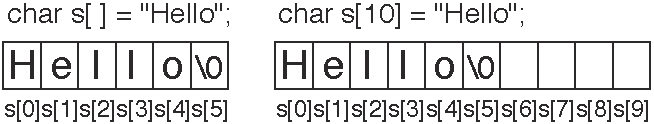
\includegraphics{hello.pdf}}
\end{figure}

\subsection{標準入力(1) : \texttt{gets}関数}
例\ref{ex:gets}を作成しコンパイルしてみよう(コンパイラによっては、「\texttt{gets} は危険だ」と警告が出るかもしれないが、実行ファイルはちゃんとできているはずである)。これを実行すると、\texttt{Input:} と表示され入力を促される。ここで、\texttt{uni}などと入力すると、\texttt{uni}と表示されてプログラムが終了する。この場合、\texttt{gets}という関数によって入力された文字列が \texttt{str} にコピーされる。注意すべきことは、\texttt{str} が \texttt{str[20]} と宣言されているので入力すべき文字列は19文字以内に限られるということである。しかし実際には、ユーザーは20字以上入力することができる。その場合、はみ出た文字は用意された領域の外に書き込まれる。もしそこが、別の変数用に使われていたら? これはとても危険なことである。\texttt{gets}を使う場合は注意が必要である\footnote{どうしても\texttt{gets}が使用したいときにはより安全性が高い\texttt{fgets}を使用せよ。}。
\begin{reidai}\label{ex:gets}
    \begin{verbatim}
#include <stdio.h>

int main(void) {
    char str[20];
    printf("Input: ");
    gets(str);
    printf("%s\n", str);
    return 0;
}
\end{verbatim}
\end{reidai}

\subsection{標準入力(2) : \texttt{scanf}関数}
例\ref{ex:gets}ではたとえ数字(19桁以下)を入力してもそれは文字列として扱われるため、数字として足し算などに用いるためには \texttt{atoi}などの関数を用いる必要がある。別の方法として、\texttt{scanf} を用いて入力した数字をそのまま数字として扱う方法を例\ref{ex:scanf}に示す(ソースコード中の \texttt{\&i} や \texttt{\&x} についている \texttt{\&} については後述する)。
\begin{reidai}\label{ex:scanf}
    \begin{verbatim}
#include <stdio.h>
#include <string.h>

int main(void) {
    int i;
    printf("Input(int): ");
    scanf("%d", &i);
    printf("%d\n", i);
    double x;
    printf("Input(double): ");
    scanf("%lf", &x);
    printf("%lf\n", x);
    return 0;
}
\end{verbatim}
\end{reidai}

\begin{renshuu}\label{prob:4-1}
    練習\ref{prob:2-2}で、標準入力から \(n\) を決定し、その答えを表示するプログラムを書きなさい。
\end{renshuu}

\section{ポインタ}

ポインタの習得はC言語の習得の中で一つの大きな壁である。はじめは訳がわからないかもしれないが、C言語の基本的な部分の一つなので、いろいろな例に触れて慣れてほしい。慣れが一番である。

\subsection{とりあえず(1)}

例\ref{ex:pointer1}を作成し実行してみよう。上手くいけば、``\texttt{q is 200 and *p is 200.}''と表示されるはずである。この例で出てくる \texttt{p} がポインタである。\texttt{int} 型のポインタを宣言するには、
\begin{quote}
    \begin{verbatim}
int *p;
\end{verbatim}
\end{quote}
のように\texttt{*}をつける。人によっては、
\begin{quote}
    \begin{verbatim}
int* p;
\end{verbatim}
\end{quote}
と宣言したほうがイメージしやすいかもしれない。つまり、\texttt{p} は \texttt{int*} 型(\texttt{int} のポインタ)ということである(しかし、2個以上のポインタを宣言するためには、\texttt{int *p, *q;} としなければならない。\texttt{int* p, q;} とすると\texttt{q}は\texttt{int}型になってしまう)。

例\ref{ex:pointer1}の \texttt{q} に格納されている\(200\)はコンピュータのメモリーのどこかに電気的に存在するはずである。その格納場所を示すものがアドレス(言うなればメモリー上の住所)であり、これを\texttt{\&q}で表す。今回はこれを\texttt{p}へと代入したので、\texttt{p}は\texttt{q}が存在する場所を指し示すようになる。

変数からそのアドレスを抽出する\texttt{\&}と対照的なのが\texttt{*}であり、これは逆にポインタからその指している先そのものを抽出する\footnote{\texttt{*}は型から1つアスタリスクを剥がし、逆に\texttt{\&}は1つ増やす、と覚えるとよい。}。\texttt{p}はあくまで\texttt{q}を指し示しているだけ(\texttt{q}が存在するアドレスの情報しか持っていない)なので、実体\texttt{q}を利用する際には\texttt{*p}とせねばならないのである。

\begin{reidai}\label{ex:pointer1}
    \begin{verbatim}
#include <stdio.h>

int main(void) {
    /* qを初期化 */
    int q = 200;
    /* qのアドレスをpに代入する */
    int* p = &q;
    /* pから指している対象そのもの(q)を取り出す */
    printf("q is %d and *p is %d.\n", q, *p);
    return 0;
}
\end{verbatim}
\end{reidai}
\begin{figure}[H]
    \centering
    \resizebox{0.50\textwidth}{!}{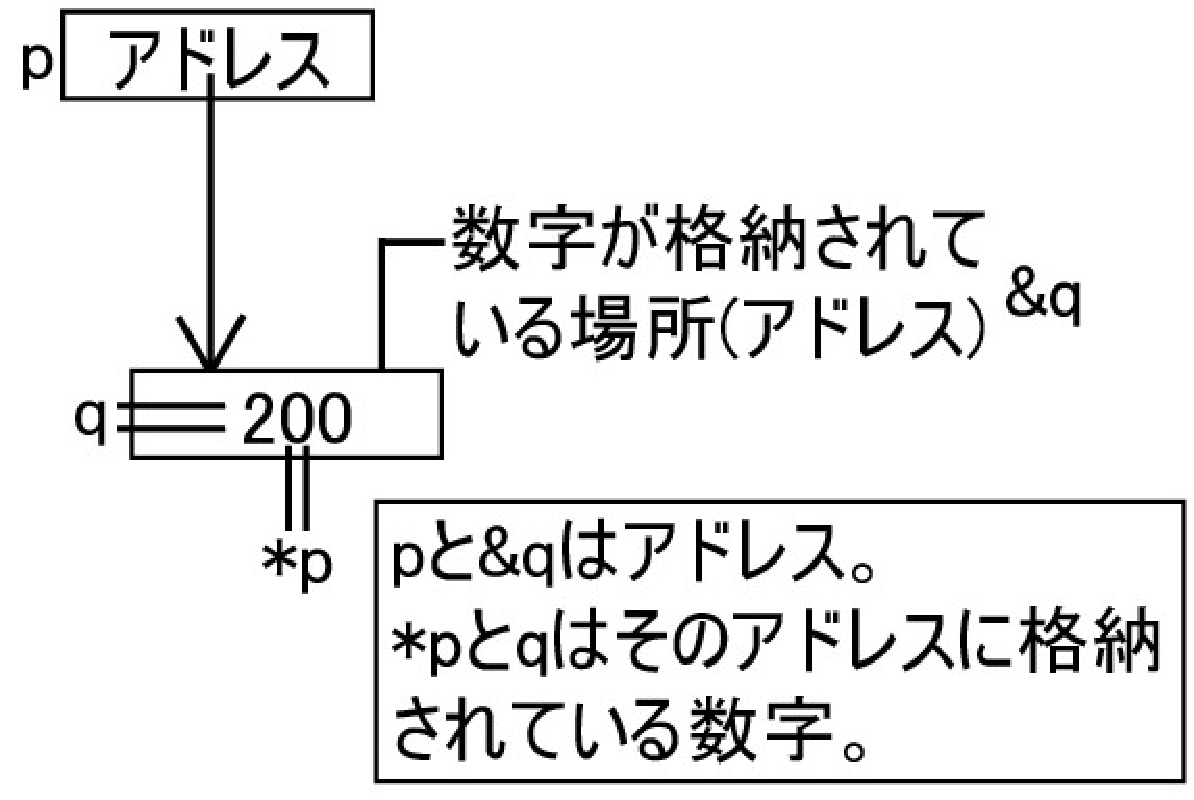
\includegraphics{pointer.pdf}}
\end{figure}

\subsection{とりあえず(2)}
では、もう一つ例を示そう。例\ref{ex:pointer2}では、\texttt{p = \&q;} によりポインタ代入を行ったので \texttt{p} というポインタで \texttt{q} にアクセスできる。ここでは、\texttt{q} に値を代入するかわりに、\texttt{*p}を用いて値を代入している。\texttt{p}はポインタで、\texttt{*p} は \texttt{p} が指している対象である\texttt{q}そのものである。
実行結果は、``\texttt{q is 300 and *p is 300.}''となる。
\begin{reidai}\label{ex:pointer2}
    \begin{verbatim}
#include <stdio.h>

int main(void) {
    int q;
    int* p = &q;
    /* 値を取得するだけでなく書き換えることもできる */
    *p = 300;
    printf("q is %d and *p is %d.\n", q, *p);
    return 0;
}
\end{verbatim}
\end{reidai} \noindent
記号\texttt{*}, \texttt{\&}などの意味と役割をもう一度復習しておこう。
\begin{table}[H]
    \centering
    \begin{tabular}{l}
        \texttt{int *p;} \\
        \texttt{int q;}
    \end{tabular}
\end{table} \noindent
の時、
\begin{table}[H]
    \centering
    \begin{tabular}{ll}
        \texttt{p}   & ポインタ (つまりどこかのアドレス) \\
        \texttt{*p}  & 実体                              \\
        \texttt{q}   & 実体                              \\
        \texttt{\&q} & \texttt{q} のアドレス
    \end{tabular}
\end{table} \noindent
である。

注意すべきことは、例\ref{ex:pointer1}や例\ref{ex:pointer2}で \texttt{p = \&q;} がない場合は \texttt{p} が\textbf{どこを指しているか未定義}であるということだ。したがって、事前の初期化なしに\texttt{*p = 300;} のように書き換えを試みたり、 \texttt{printf} 内で \texttt{*p} を表示させるのは危険である。何が起こるか分からない。

この節では、静的に宣言された変数を指すためにポインタを用いてきたが、より高度な使い方については\ref{sec:clang:malloc}節で紹介する。

\subsection{ポインタと配列}
\label{sec:C:pointer-array}
ポインタと配列には密接な関係がある。
\begin{quote}
    \begin{verbatim}
int array[10];
\end{verbatim}
\end{quote}
と宣言した場合、\texttt{array[0]} や \texttt{array[5]} などで配列の要素にアクセスすることができた。実は、\texttt{array} だけでも意味を持つ。\texttt{array} は配列型 (\texttt{int[10]} 型) の変数で、プログラムコード中に登場した時は、大抵の状況では、自動的に ``配列の先頭要素のアドレス''に暗黙的に変換されて解釈される。つまり、\texttt{array} は \texttt{array[0]} へのポインタとして解釈され、\texttt{*array} は \texttt{array[0]}を意味する。さらに、ポインタに整数を足すとその数だけ先の要素を指すようになる。例えば\texttt{array + 2}は\texttt{array[2]} へのポインタであり、\texttt{*(array + 2)} は \texttt{array[2]}と等価である。

では、例\ref{ex:pointer-array}を見てみよう。\texttt{strlen} という関数は \texttt{string.h} 内で宣言されている文字列の長さを返す関数である。最初の \texttt{for} 文は文字型の配列 \texttt{str} の中身を順番に書き出している。次の \texttt{for} 文がポイントである。ここではまず文字型のポインタ \texttt{p} に文字型の配列 \texttt{str} の先頭ポインタ \texttt{str} を代入している。そして、文字型の実体である \texttt{*p} が \texttt{\textbackslash 0} でない場合はその \texttt{*p} を表示し、ポインタ \texttt{p} の指す部分を一つ進めている。これを \texttt{*p} が \texttt{\textbackslash 0} になるまで繰り返すことで、最初の \texttt{for} 文と同じ結果を表示できるというわけである。
\begin{reidai}\label{ex:pointer-array}
    \begin{verbatim}
#include <stdio.h>
#include <string.h>

int main(void) {
    const char str[] = "ABCDE";
    const int num = strlen(str);
    for (int i = 0; i < num; ++i) {
        printf("%c", str[i]);
    }
    printf("\n");
    for (const char* p = str; *p != '\0'; ++p) {
        printf("%c", *p);
    }
    printf("\n");
    return 0;
}
\end{verbatim}
\end{reidai}

\subsection{\texttt{const}とポインタについて}
ポインタを介して変数を操作出来るのは便利な反面、意図せず書き換えてしまった結果バグを生じたり、そもそも\texttt{const}のついた変数をどうやってポインタで参照するのか(うっかり書き換えてしまったりしないのか)といった問題が生じる。これを解決するのが\texttt{const}つきのポインタである。

\begin{table}[H]
    \centering
    \begin{tabular}{lll}
        型                         & ポインタ自体を変更できるか & そのポインタから実体を変更できるか \\
        \texttt{type*}             & \(\bigcirc\)               & \(\bigcirc\)                       \\
        \texttt{const type*}       & \(\bigcirc\)               & \(\times\)                         \\
        \texttt{type* const}       & \(\times\)                 & \(\bigcirc\)                       \\
        \texttt{const type* const} & \(\times\)                 & \(\times\)
    \end{tabular}
\end{table} \noindent

少し難しい概念ではあるが、バグを防ぐ上で非常に強力であるので困ったときにはぜひ使ってみてほしい。
\begin{renshuu}\label{prob:5-1}
    次のプログラムの \texttt{printf} の部分を配列ではなく、ポインタを使ったものに書き換えなさい(\texttt{array} を使っても、あるいは、\texttt{int *p;} を加えてもよい)。
\begin{quote}
\begin{verbatim}
#include <stdio.h>

int main(void)
{
    int array[10];
    for (int i = 0; i < 10; ++i) {
        array[i] = i * i;
    }
    for (int i = 0; i < 10; ++i) {
        printf("array[%d] = %d\n", i, array[i]);
    }
    return 0;
}
\end{verbatim}
\end{quote}
\end{renshuu}

\section{複素数}
\label{sec:C:complex}
量子力学などの数値計算では複素数を用いることも多い。
Cにおいても複素数変数を扱うための型が用意されている\footnote{複素数の機能はC11で必須でなくなってしまった。}。
\begin{table}[H]
    \centering
    \begin{tabular}{ll}
        \texttt{float complex}  & 単精度複素数型 \\
        \texttt{double complex} & 倍精度複素数型
    \end{tabular}
\end{table} \noindent
複素数型を使うためには、プログラムの冒頭で\texttt{complex.h}ヘッダファイルを読み込む必要がある。\texttt{csin}, \texttt{cexp}, \texttt{clog}などの複素初等関数も用意されている\footnote{単精度複素数の場合は、\texttt{csinf}, \texttt{cexpf}, \texttt{clogf}のように関数名の後に \texttt{f}を付ける。}。以下の例では、\(\exp(i\pi)\)の計算を行っている。
\begin{reidai}\label{ex:complex}
    \begin{verbatim}
#include <complex.h>
#include <math.h>
#include <stdio.h>

int main(void) {
    const double complex x = 0 + 1 * I; /* 虚数単位 */
    const double complex y = cexp(x * M_PI);
    printf("i = (%lf,%lf)\n", creal(x), cimag(x));
    printf("e^{i*pi} = (%lf,%lf)\n", creal(y), cimag(y));
    return 0;
}
\end{verbatim}
\end{reidai} \noindent
虚数単位は大文字の \texttt{I} と書く。あるいは、大文字の\texttt{CMPLX}関数\footnote{単精度複素数の場合、\texttt{CMPLXF}。}を使って、\texttt{x = CMPLX(0,1)} のように表すこともできる。複素数の実部、虚部を取り出すにはそれぞれ、\texttt{creal}, \texttt{cimag}を使う。
絶対値、偏角、複素共役はそれぞれ、\texttt{cabs}, \texttt{carg}, \texttt{conj}である\footnote{単精度複素数の場合、それぞれ \texttt{crealf}, \texttt{cimagf}, \texttt{cabsf}, \texttt{cargf}, \texttt{conjf}である。}。

\clangpara{\texttt{tgmath.h}について}
C言語では関数名に重複があってはならないので、数学関数が型ごとに違う名前を持っている。これをいちいち切り替えるのは面倒であるが、新しい規格においては勝手に引数の型を読み取って適切な関数を呼び出してくれる便利な\texttt{tgmath.h}というものが追加されている。

\section{関数}
\label{sec:C:function}

\ref{sec:C:basic}節でC言語の基本構造を説明したが、\texttt{main(){...}} だけでプログラムを書くことはほとんどない。大きなプログラムになればなるほど関数化を行い、役割分担をはっきりさせるのがよい。

\subsection{あまり良くない例}
例\ref{ex:non-function}は円の面積の計算するために直接その公式を書いている。しかし、何度も何度も円の面積を計算したいとき、半径を入力すれば面積が返ってくるような関数があれば非常に便利である。
\begin{reidai}\label{ex:non-function}
    \begin{verbatim}
#include <math.h>
#include <stdio.h>

int main(void) {
    const double radius = 2.0;
    const double area = radius * radius * M_PI;
    printf("Radius: %lf, Area: %lf\n", radius, area);
    return 0;
}
\end{verbatim}
\end{reidai}

\subsection{関数化}
では、例\ref{ex:non-function}を例\ref{ex:function1}のように変更してみよう。このような小さなプログラムでは関数化の効力は乏しいが、大きくなればなるほど、また複雑になればなるほど、その効力は絶大になる。例\ref{ex:function1}では、\texttt{circle\_area} という関数が定義されている。この関数では、double型の値を引数として受け取り、面積を計算してその値を戻り値にしている。

\begin{reidai}\label{ex:function1}
    \begin{verbatim}
#include <math.h>
#include <stdio.h>

double circle_area(double r) {
    return r * r * M_PI;
}

int main(void) {
    const double radius = 2.0;
    const double area = circle_area(radius);
    printf("Radius: %lf, Area: %lf\n", radius, area);
    return 0;
}
\end{verbatim}
\end{reidai}

通常、関数は使う前に``宣言''する必要がある。(例\ref{ex:function1}は特殊な場合であり、関数の定義が宣言を兼ねている)
きちんと宣言を行うときには、例\ref{ex:function2}のように関数の引数名と処理部分がない不完全な定義のようなもの(これが宣言の書式である)を書く必要がある。

関数を使用する際には使用箇所から宣言が見えるようにしておく必要があるが、逆に宣言さえ見えていれば定義はどこにあっても構わない\footnote{より厳密に言うならば、\texttt{gcc}に渡す\texttt{.c}ファイルのどれか、あるいはリンクするライブラリに定義が含まれていれば問題ない。}。
例\ref{ex:function2}は、``宣言は見えるが、定義は見えない''場合の典型例になっている。

\begin{reidai}\label{ex:function2}
    \begin{verbatim}
#include <math.h>
#include <stdio.h>

double circle_area(double);

int main(void) {
    const double radius = 2.0;
    const double area = circle_area(radius);
    printf("Radius: %lf, Area: %lf\n", radius, area);
    return 0;
}

double circle_area(double r) {
    return r * r * M_PI;
}
\end{verbatim}
\end{reidai}

\subsection{ポインタを引数にする関数}

例\ref{ex:function1}では関数の返り値が面積の一つだけであった。しかし、例えば割り算で商と余りを返したい場合、例\ref{ex:function1}のような関数ではうまく実現できない。なぜなら、戻り値は1個しか指定できないからである。これを解決するには、ポインタを引数とする関数を作り、あらかじめ準備しておいた答えを入れる変数を関数の引数にポインタとして渡し、関数内でそこに答えを入れてもらって関数の外で受け取るという方法が有効である。重要な点は、ポインタでなければ関数内で代入した値を関数の外で使うことはできないということである。

例\ref{ex:function-pointer}では、まず\texttt{main}で答えを入れてもらうための \texttt{shou} と \texttt{amari} という箱(変数)を準備している。次に、そのポインタ(アドレス)を関数\texttt{division}に渡している。そして、\texttt{division}内で答えを代入してもらい、関数の外で\texttt{printf}を用いて答えを表示している。\texttt{division} という関数の先頭にある\texttt{void}という型は(返り値の形では)何も返さないことを示すためのものである。
\begin{reidai}\label{ex:function-pointer}
    \begin{verbatim}
#include <stdio.h>

void division(int divident, int divisor, int* const quotient,
    int* const residual) {
    *quotient = divident / divisor;
    *residual = divident % divisor;
}

int main(void) {
    const int josuu = 3;
    const int hi_josuu = 13;
    int shou, amari;
    division(hi_josuu, josuu, &shou, &amari);
    printf("%d / %d = %d ... %d\n", hi_josuu, josuu, shou, amari);
    return 0;
}
\end{verbatim}
\end{reidai} \noindent
ポインタを使う理由がはっきりと分からない場合は、例\ref{ex:function-non-pointer}を作って実行してみてほしい。間違った答えが表示されるだろう。なぜなら、この場合 \texttt{division} という関数では、\texttt{quotient}と\texttt{residual}という二つの一時変数が生成され、それらに計算結果が代入された直後に破棄されるからである。一時変数は関数の処理が終了すると同時に破棄され、値は \texttt{main} の中の \texttt{shou} と \texttt{amari} には引き継がれない\footnote{ブロック中での変数定義の挙動を思い出そう。}。このため、関数に外部から値を渡すだけであれば、例\ref{ex:function-non-pointer}のような引数の宣言方法でよい(「値渡し」と呼ぶ)が、内での計算結果を関数の外で使いたい場合は、ポインタを使って変数のアドレスを渡す(「ポインタ渡し」と呼ぶ)必要がある。
\begin{reidai}\label{ex:function-non-pointer}
    \begin{verbatim}
#include <stdio.h>

void division(int divident, int divisor, int quotient, int residual) {
    quotient = divident / divisor;
    residual = divident % divisor;
}

int main(void) {
    const int josuu = 3;
    const int hi_josuu = 13;
    int shou, amari;
    division(hi_josuu, josuu, shou, amari);
    printf("%d / %d = %d ... %d\n", hi_josuu, josuu, shou, amari);
    return 0;
}
\end{verbatim}
\end{reidai}

\subsection{関数ポインタ}
ポインタはメモリ上にある変数を指し示すものであったが、実は関数そのものもメモリ上に配置されているのでポインタが使える。例えば\texttt{int}を受け取って\texttt{double}を返す関数用のポインタ\texttt{p}を宣言したいときには\texttt{double (*p)(int);}と書けばよい\footnote{変数宣言らしからぬ特殊な記法であるが、これであっている。}。

関数ポインタを使うと``関数を引数として受け取る関数''\footnote{いわゆる汎関数のようなものを作ることができる。}が実現でき、うまく使うと非常に強力である。

\subsection {Fortranの関数や手続きの利用}

LAPACK\footnote{行列の対角化、連立1次方程式の求解など線形計算を行うライブラリ。ほぼ全ての計算機で利用可能である。}などの多くのライブラリがFortranで書かれている。これらと同等の機能を持つ関数をCやC\texttt{++}で作ることもできるが、既に存在するのであればそちらを使った方が便利である。ここでは、C言語の中からFortranの関数や手続きを呼ぶ方法を簡単に紹介する。

Fortranの関数や手続きの名前をC言語から呼ぶためには、その名前をすべて小文字にして、最後に\_ (下線)を付けなければならない。また、関数などの引数の型も適切に読み変える必要がある。例えば、
\begin{reidai}\label{ex:fort}
    \begin{verbatim}
      Real*8 CALC(I, X, Y)
      Interger*4 I
      Real*4 X
      Real*8 Y
\end{verbatim}
\end{reidai} \noindent
というFortranの関数が存在するとする。このときCでは以下のような宣言を書く必要がある。
\begin{reidai}
    \begin{verbatim}
extern double calc_(int*, float*, double*);

int main(void) {
    int i = 10;
    float x = 20.0F;
    double y = 30.0;
    double ret = calc_(&i, &x, &y);
    return 0;
}
\end{verbatim}
\end{reidai} \noindent
全ての引数をポインタ渡しとしなければならないことに特に注意せよ。コンパイルはC (\texttt{gcc})とFortran (\texttt{gfortran})で別々に行い、最後にリンクすればよい\footnote{LAPACKはすでにコンパイル済みなので\texttt{gfortran}は必要ない。リンクの方法については\ref{ex:ext_lib}を見よ。}。

\section{構造体}
データ構造を取り扱うためには構造体を用いる。

例\ref{ex:struct1}を見てほしい。個人のデータを取り扱うために \texttt{personal\_data} という一つの箱を準備している。これが構造体である。もし構造体を使わなければ、同じ内容のプログラムを実現するために複数の配列を準備する必要が出てくる。これは見た目にも格好悪いし、拡張性も乏しく複雑になる。例\ref{ex:struct1}では、\texttt{struct personal\_data pdata;} で \texttt{pdata} を構造体とし宣言している。少し分かりにくいかもしれないが、\texttt{int n;}と比べてみると、\texttt{int} と ``\texttt{struct personal\_data}''が同じ立場であって、\texttt{int} と ``\texttt{struct}''が同じ立場というわけではないことに注意してほしい。\texttt{int} という型はあらかじめC言語で決められた型なのに対し、構造体は自分が好きなように使いやすいように決めた型だと考えても構わない。つまり、``\texttt{struct personal\_data}''型というものを自分で作ったと考えるのである。そうすれば、\texttt{struct personal\_data pdata;} という使い方も理解できるはずである。

構造体内の各データには、ドット演算子 (\texttt{.}) を使ってアクセスする。また、年齢を文字列 \texttt{buffer[16]} として受け取っているため、\texttt{atoi} 関数を用いて数字に変換している。\texttt{atoi} は文字列を整数に変換する関数である。詳しくはコマンドラインで \texttt{man atoi} としてみよ。
\begin{reidai}\label{ex:struct1}
    \begin{verbatim}
#include <stdio.h>
#include <stdlib.h>

struct personal_data {
    char family_name[16];
    char given_name[16];
    int age;
};

int main(void) {
    struct personal_data pdata;
    char buffer[16];
    printf("Input family name: ");
    gets(pdata.family_name);
    printf("Input given name: ");
    gets(pdata.given_name);
    printf("Input age: ");
    gets(buffer);
    pdata.age = atoi(buffer);
    printf("Family Name = %s\n", pdata.family_name);
    printf("Given  Name = %s\n", pdata.given_name);
    printf("Age         = %d\n", pdata.age);
    return 0;
}
\end{verbatim}
\end{reidai} \noindent
構造体を指すポインタの場合は、次の例\ref{ex:struct2}のように、アロー演算子 (\texttt{->}) でその構造体の要素にアクセスすることができる。例題中の\texttt{qdata->p[0]}は\texttt{(*qdata).p[0]}と等価である。ちなみに、この例の構造体は粒子の質量と運動量を格納している。
\begin{reidai}\label{ex:struct2}
    \begin{verbatim}
#include <stdio.h>

struct particle_data {
    double mass;
    double p[3]; /* Momentum */
};

int main(void) {
    const struct particle_data pdata = { 0.14, { 1.2, 1.3, 1.4 } };
    const struct particle_data* const qdata = &pdata;
    printf("Mass = %lf\n", qdata->mass);
    printf("Momentum = (%lf, %lf, %lf)\n", qdata->p[0], qdata->p[1],
        qdata->p[2]);
    return 0;
}
\end{verbatim}
\end{reidai}

\begin{renshuu}\label{prob:7-1}
    ``月'', ``日'', ``1月1日からの日数(うるう年ではない)''を構成要素とする構造体を作って、``月'' と ``日''を標準入力から入力すれば、自動的に ``1月1日からの日数''の部分を埋め、最後にそれを表示して終了するプログラムを書きなさい。
\end{renshuu}

\section{ファイルの取り扱い}

ファイルから数字を読みこんだり、ファイルに結果を書き込んだりするプログラムを紹介する。ここで挙げた例だけでも基本的なことはできるはずである。より詳しく知りたい場合は参考書などを参照してほしい。

\subsection{ファイルから数字の読み込み}

例\ref{ex:file-read1}がファイルから数字を読み込むときの雛型となる。まず、\texttt{FILE *fp;} でファイルを取り扱うための構造体を宣言する。\texttt{char *filename}の部分でファイル名を宣言する。そして、\texttt{fopen}でファイルを開く。(\texttt{"r"} はread (読み取り専用)でファイルを開くことを示す。) \texttt{if(fp==NULL){}} の部分はエラーが起こったときに処理され、プログラムを強制終了させる\footnote{\texttt{NULL}は特別なポインタで、``なにか異常が起きた結果、ポインタが有効な場所を指さずに宙ぶらりんになっている''ことを表現するためにある。今回の例ではファイルが何らかの原因で読み取れなかったときに\texttt{NULL}が返ってくる。}。\texttt{fscanf}で順番にファイルに書かれている数字を\texttt{double}型で読み取っている。\texttt{fscanf}の使い方は、
\begin{quote}
    \begin{verbatim}
fscanf(ファイル構造体のポインタ, "フォーマット", &変数1, &変数2, ......);
\end{verbatim}
\end{quote}
で、ファイル構造体のポインタ部分以外は \texttt{scanf} と同じである。最後に \texttt{fclose(fp);} でファイルを閉じている。
\begin{reidai}\label{ex:file-read1}
    \begin{verbatim}
#include <stdio.h>
#include <stdlib.h>

double product(double x1, double y1, double x2, double y2) {
    return x1 * x2 + y1 * y2;
}

int main(void) {
    const char filename[] = "vectors.txt";
    FILE* fp = fopen(filename, "r");
    if (fp == NULL) {
        printf("Can't open file %s\n", filename);
        exit(1);
    }
    double x1, y1, x2, y2;
    /* read first line */
    fscanf(fp, "%lf %lf\n", &x1, &y1);
    /* read second line */
    fscanf(fp, "%lf %lf\n", &x2, &y2);
    fclose(fp);
    const double p = product(x1, y1, x2, y2);
    printf("Product of (%lf,%lf) and (%lf,%lf) is %lf\n", x1, y1, x2, y2, p);
    return 0;
}
\end{verbatim}
\end{reidai} \noindent
例\ref{ex:file-read1}を実行するためには、\texttt{vectors.txt}というファイル名で以下のような内容の入力ファイルも作っておく必要がある。
\begin{quote}
    \begin{verbatim}
 1.0    2.0
-1.5    3.5
\end{verbatim}
\end{quote}
例\ref{ex:file-read1}のデータを読み込む部分を、例\ref{ex:file-read2}のように \texttt{while} を使って書き直してみよう。こちらの方がファイルに存在するデータを最後まで読み取るという点で、より汎用性が高い。\texttt{fscanf}はデータの読み込みに失敗すると\texttt{EOF}を返すので、\texttt{EOF}が返ってくるまで読み込みを繰り返している\footnote{\texttt{while}の条件式チェックと読み込みを同時に行っている。}。
\begin{reidai}\label{ex:file-read2}
    \begin{verbatim}
#include <stdio.h>
#include <stdlib.h>

#define N_DATA 100

int main(void) {
    const char filename[] = "vectors.txt";
    FILE* fp = fopen(filename, "r");
    if (fp == NULL) {
        printf("Can't open file %s\n", filename);
        exit(1);
    }
    double x[N_DATA][2];
    int index = 0;
    /* read data */
    while (fscanf(fp, "%lf %lf\n", &x[index][0], &x[index][1]) != EOF) {
        printf("Data %d : (%lf, %lf)\n", index, x[index][0], x[index][1]);
        ++index;
    }
    fclose(fp);
    return 0;
}
\end{verbatim}
\end{reidai}

\subsection{ファイルへの数字の書き出し}

例\ref{ex:file-write}がファイルへ数字を書き出すときの雛型である。ファイルを開くところまでは例\ref{ex:file-read1}とはほぼ同じで、違う点は \texttt{fopen} の第二引数が \texttt{"r"} ではなく \texttt{"w"} (書きこみ)である点である。書き出すときには \texttt{fprintf} という関数を使っている。\texttt{fprintf} の使い方は、
\begin{quote}
    \begin{verbatim}
fprintf(ファイル構造体のポインタ, "フォーマット", 変数1, 変数2, ......);
\end{verbatim}
\end{quote}
で、ファイル構造体のポインタ部分以外は \texttt{printf} と同じである。最後に、\texttt{fclose(fp);} でファイルを閉じる。
\begin{reidai}\label{ex:file-write}
    \begin{verbatim}
#include <math.h>
#include <stdio.h>
#include <stdlib.h>

double circle_area(double r) {
    return r * r * M_PI;
}

int main(void) {
    const char filename[] = "circle_area.txt";
    FILE* fp = fopen(filename, "w");
    if (fp == NULL) {
        printf("Can't open file %s\n", filename);
        exit(1);
    }
    for (int i = 1; i <= 10; ++i) {
        const double radius = i;
        const double area = circle_area(radius);
        fprintf(fp, "%lf -> %lf\n", radius, area);
    }
    fclose(fp);
    return 0;
}
\end{verbatim}
\end{reidai}

\section{その他の制御文}

\texttt{for}, \texttt{while}以外の制御文の書式を紹介する。

\subsection{\texttt{switch}-\texttt{case}文}

1の場合にはAを、2の場合にはBを、3の場合にはCを、という風に条件分岐をしたい場合に、\texttt{switch}-\texttt{case}文を用いる。
\begin{reidai}\label{ex:case}
    \begin{verbatim}
#include <stdio.h>
#include <string.h>

int main(void) {
    int i;
    printf("Input(int): ");
    scanf("%d", &i);
    printf("%d / 3 no amari ha ", i);
    switch (i % 3) {
    case 1:
        printf("1 desu.\n");
        break;
    case 2:
        printf("2 desu.\n");
        break;
    default:
        printf("0 desu.\n");
    }
    return 0;
}
\end{verbatim}
\end{reidai} \noindent
今回は\texttt{i \% 3}をチェックの対象とし、上から\texttt{1}のとき、\texttt{2}のとき、それ以外の順で処理を記述している。もし例\ref{ex:case}の \texttt{switch}-\texttt{case} 文中に \texttt{break;} がないと、\texttt{case 1:} の場合は \texttt{case 2:} の部分も \texttt{default:} の部分も実行してしまうことに注意\footnote{\texttt{-Wextra}をつけていればきちんと警告が出るので安心してよい。}。(\texttt{case 1:} 以下の部分から下の部分をすべて実行する。)したがって、\texttt{case 2:} の直前で抜けるためには \texttt{break;} が必要となる。実際に \texttt{break;} を削除して試してみよう。この場合は常に \texttt{...0 desu.} が表示されるはずである。

\texttt{switch}-\texttt{case} 文を簡単にまとめると、次のようになる。
\begin{quote}
    \begin{verbatim}
switch (X) {
  case A:  ブロック1
  case B:  ブロック2
  ...
  default: ブロックN
}
\end{verbatim}
\end{quote}
\texttt{switch}文に処理が到達すると、\texttt{X}が上から順に\texttt{case}と照合されていき、一致したところでブロックに入る。\texttt{switch}から抜けるには\texttt{break;}を使用する。\texttt{case}はいくつあっても構わない。

\subsection{\texttt{do}-\texttt{while}文}

\texttt{while} 文と同様に、ある条件が満たされている場合に繰り返しを行うために \texttt{do}-\texttt{while} 文を使う。\texttt{while} 文と違う点は、条件の判定する``タイミング''である。\texttt{while} 文の場合は、まず条件を判定し、満足していれば\texttt{while} 内を実行するが、\texttt{do}-\texttt{while} 文の場合は、まず\texttt{do}-\texttt{while} 内を実行してから条件を判定する。したがって、\texttt{while} 文の場合は \texttt{while} 内を1度も実行しない場合があるが、\texttt{do}-\texttt{while} 文の場合は必ず1度は \texttt{do}-\texttt{while} 内を実行する。
\begin{reidai}\label{ex:do-while}
    \begin{verbatim}
#include <stdio.h>

int main(void) {
    int i = 100;
    int sum = 0;
    do {
        sum += i;
        --i;
    } while (i != 0);
    printf("sum of integers from 100 to 1 is %d\n", sum);
    return 0;
}
\end{verbatim}
\end{reidai} \noindent
例\ref{ex:do-while}のように、\texttt{while()} の後ろの \texttt{;} を忘れないこと。
\texttt{do}-\texttt{while} 文の基本的な動作は次のようになる。
\begin{quote}
    \begin{verbatim}
do {
  ブロック
} while (A);
\end{verbatim}
\end{quote}
\texttt{do}に処理が到達すると、``ブロックを実行\(\rightarrow\)\texttt{A}をチェックし、偽なら抜ける''の操作が繰り返される。

\section{コマンドライン引数の受け渡し}
\texttt{main}文には、\texttt{int main(void)} 以外に、\texttt{int main(int, char**)}, あるいは \texttt{int main(int, char*[])} という書き方がある。これらの書式を利用すれば、実行時に引数を与えてそれを利用することができる。つまり、今までは
\begin{commandline2}
    \prompt \underline{./a.out}
\end{commandline2} \noindent
として実行していたが、これを利用すれば、
\begin{commandline2}
    \prompt \underline{./a.out input.data output.data}
\end{commandline2} \noindent
のように、ファイル名や数値などをコマンドライン引数としてプログラムに渡すことができる。

\subsection{ポインタ配列}

新しい\texttt{main}関数の説明の前に、引数の受け渡しに使われているポインタ配列に関して説明しておこう。ポインタ配列は、名前通り、ポインタを要素とする配列(\texttt{char*[]})である。配列はポインタを使ってアクセス可能なので、``ポインタのポインタ'' (\texttt{char**})と同様に使うことができる。
\begin{reidai}\label{ex:pointers-array}
    \begin{verbatim}
#include <stdio.h>

int main(void) {
    char* name0 = "Alice";
    char* name1 = "Bob";
    char* name2 = "Claire";
    char* name3 = "David";
    char* name[4];
    name[0] = name0;
    name[1] = name1;
    name[2] = name2;
    name[3] = name3; /* A */
    /* B */
    for (int i = 0; i < 4; ++i) {
        printf("Name%d : %s\n", i, name[i]);
    }
    /* C */
    for (int i = 0; i < 4; ++i) {
        printf("Name%d : %c, %s\n", i, **(name + i), *(name + i));
    }
    return 0;
}
\end{verbatim}
\end{reidai} \noindent
例\ref{ex:pointers-array}の結果は以下のようになる。
\begin{quote}
    \begin{verbatim}
Name0 : Alice
Name1 : Bob
Name2 : Claire
Name3 : David
Name0 : A, Alice
Name1 : B, Bob
Name2 : C, Claire
Name3 : D, David
\end{verbatim}
\end{quote}
まず、\texttt{name[0]} の型は \texttt{char*} なので、\texttt{name0} の値などを代入することができる。Aの時点で、\texttt{name} というポインタ配列の各要素にアドレスの代入したことになる。つまり、
\begin{quote}
    \begin{verbatim}
name[0] = "Alice"という文字列の先頭アドレス
name[1] = "Bob"という文字列の先頭アドレス
name[2] = "Claire"という文字列の先頭アドレス
name[3] = "David"という文字列の先頭アドレス
\end{verbatim}
\end{quote}
となっている。したがって、Bの \texttt{for} 文では、\texttt{printf} に文字列の先頭アドレスを渡すことで、名前を表示することができる。次に、Cの \texttt{for} 文である。これは若干混乱を招くが、次が理解出来れば、何とかクリアできるだろう。
\begin{table}[H]
    \centering
    \begin{tabular}{r@{ = }c@{ = }l}
        \texttt{name}   & 文字へのポインタのポインタ & \texttt{char**} 型                      \\
        \texttt{*name}  & 文字へのポインタ           & \texttt{char*} 型                       \\
        \texttt{**name} & 文字                       & \texttt{char} 型 (※ 文字列ではなく文字)
    \end{tabular}
\end{table}
\texttt{printf} は \texttt{\%s} で文字列の先頭アドレス、つまり、\texttt{char*} を受け取り、\texttt{\%c} で文字型そのもの、つまり、\texttt{char} を受け取る。また、\texttt{name + i} という書き方は\texttt{\&(name[i])}とほぼ等価である。

\subsection{新しい\texttt{main}関数}

例\ref{ex:new-main}がコマンドライン引数を受け取ることのできる \texttt{main}関数の例である。\texttt{int main(int argc, char* argv[])}は、\texttt{int main(int argc, char** argv)}と書いても同じである。好きなほうを使えばよい。
また、伝統的に \texttt{argc} と \texttt{argv} という名前を使っているが、他の変数名でも構わない。
\begin{reidai}\label{ex:new-main}
    \begin{verbatim}
#include <stdio.h>
#include <stdlib.h>

int main(int argc, char* argv[]) {
    if (argc != 3) {
        /* A */
        printf("Usage: sumXY InputFile OutputFile\n");
        exit(1);
    }
    const char* const InputFileName = argv[1];
    const char* const OutputFileName = argv[2];
    /* input */
    FILE* fp = fopen(InputFileName, "r");
    if (fp == NULL) {
        printf("Can't open file %s\n", InputFileName);
        exit(1);
    }
    int counter = 0;
    double x, y;
    double sumX = 0.0, sumY = 0.0;
    /* read data */
    while (fscanf(fp, "%lf %lf\n", &x, &y) != EOF) {
        sumX += x;
        sumY += y;
        ++counter;
    }
    fclose(fp);
    /* output */
    fp = fopen(OutputFileName, "w");
    if (fp == NULL) {
        printf("Can't open file %s\n", OutputFileName);
        exit(1);
    }
    /* write results */
    fprintf(fp, "Number of Data = %d\n", counter);
    fprintf(fp, "X Sum = %lf\n", sumX);
    fprintf(fp, "Y Sum = %lf\n", sumY);
    fclose(fp);
    return 0;
}
\end{verbatim}
\end{reidai} \noindent
例\ref{ex:new-main}を\ref{ex:new-main}cという名前で保存し、次のようにコンパイルする。
\begin{commandline2}
    \prompt \underline{gcc -o sumXY \ref{ex:new-main}c -Wall -Wextra}
\end{commandline2} \noindent
\texttt{sumXY}は例\ref{ex:new-main}のAの部分の\texttt{printf}のメッセージに合わせてある。次のようにして実行してみよう。
\begin{commandline2}
    \prompt \underline{./sumXY}\\
    Usage: sumXY InputFile OutputFile
\end{commandline2} \noindent
このとき\texttt{InputFile}, \texttt{OutputFile}の二つのコマンドライン引数が必要であるというエラーが表示される。例\ref{ex:new-main}のAの部分を変更することで、エラーメッセージは変更することができる。次のように実行しても同じメッセージが出力されるはずである。
\begin{commandline2}
    \prompt \underline{./sumXY input.dat}
\end{commandline2} \noindent
\begin{commandline2}
    \prompt \underline{./sumXY input.dat output.dat 10}
\end{commandline2} \noindent
一番目の例は引数が足りず、二番目の例は引数が多すぎるからである。例\ref{ex:new-main}では \texttt{argc} が3以外ならエラーメッセージを表示するようにしてあるが、
\begin{commandline2}
    \prompt \underline{./sumXY input.dat output.dat 10}
\end{commandline2} \noindent
は3個の引数だからエラーが出るのはおかしい、と考えるかもしれない。しかし、これは正しい動作である。なぜなら、引数としてプログラム名(\texttt{./sumXY})も1個と数えられるからである\footnote{\texttt{argv[0]}を用いると、例\ref{ex:new-main}のAのエラーメッセージは \texttt{printf("Usage: \%s InputFile OutputFile\textbackslash n", argv[0]);}と書くことができる。このようにしておくと、プログラム名をあらかじめソースコードに明示的に書き込む(「ハードコーディング」と呼ぶ)必要がなくなる。}。つまり、二番目の例では、\texttt{argc}の値は4であり、\texttt{argv}の中身は
\begin{quote}
    \begin{verbatim}
argv[0] = "./sumXY"の先頭アドレス
argv[1] = "input.dat"の先頭アドレス
argv[2] = "output.dat"の先頭アドレス
argv[3] = "10"の先頭アドレス
\end{verbatim}
\end{quote}
となっている。

\texttt{argc}が想定していた値と異なる場合、配列\texttt{argv}の有効範囲からはみ出した部分を参照して致命的なバグを発生させることがあるので、\texttt{argc}のチェック機構は面倒でもつけるようにしたほうがよい。

最後に、1行に2個の数字で10行程度書いた\texttt{input.dat}を作成し、次のように実行してみよう。\texttt{output.dat}に結果が書き込まれているはずである。
\begin{commandline2}
    \prompt \underline{./sumXY input.dat output.dat}
\end{commandline2}

\section{動的な配列の確保: \texttt{malloc}と\texttt{free}}
\label{sec:clang:malloc}

これまで、ポインタはあらかじめ確保した領域に対してのみ使ってきた。しかし、実行時に、入力値あるいは計算結果を反映して、50個のデータを取り扱いたいときもあれば、100個のデータを取り扱いたいときもある。もちろん、配列を利用してあらかじめ十分な大きさの領域(いまの場合は100個以上の数)を確保しておけばよいかもしれないが、平均的に10個ぐらいしか利用しないのに、たまに100個の場合があるからといって常に100個分の領域を確保しておくことは、無駄のように思える。これを回避するために、動的に、つまり、実行時に領域を確保する手段がある。これが、\texttt{malloc} (\textbf{m}emory \textbf{alloc}cationの略)である。

\subsection{\texttt{malloc}の使い方}

例\ref{ex:malloc}に\texttt{malloc}の使い方の雛型を示す\footnote{簡単のため、コマンドライン引数のチェックは行っていない。実際のプログラムでは、配列を確保する前に確保しようとしているサイズを確認すべきである。}。\texttt{malloc}は領域を確保できた場合はその領域の先頭アドレスを返すが、領域が確保できなかった場合は\texttt{NULL}を返す。\texttt{NULL}の場合は、何らかのエラー処理を行う必要がある。例\ref{ex:malloc}では、プログラムを強制的に終了している。\texttt{sizeof}関数は型の大きさ(バイト数)を調べる関数である。この場合は\texttt{int}の大きさ(通常4)を調べている。\texttt{double}を大きさを調べたい場合は\texttt{sizeof(double)}のように使う。例\ref{ex:malloc}では、\texttt{int} の領域を \texttt{n\_element} 個分確保したいので、\texttt{sizeof(int) * n\_element}を\texttt{malloc}に与えている\footnote{\texttt{malloc}はあらゆる型に対して使えるように要素数ではなくバイト数単位で必要メモリ量を指定する設計になっている。引数に\(0\)を与えてはならない。}。
\begin{reidai}\label{ex:malloc}
    \begin{verbatim}
#include <stdio.h>
#include <stdlib.h>

int main(int argc, char* argv[]) {
    const int n_element = atoi(argv[1]);
    int* array = (int*)malloc(sizeof(int) * n_element);
    if (array == NULL) {
        printf("Can't allocate memory.\n");
        exit(1);
    }
    for (int i = 0; i < n_element; ++i) {
        array[i] = i * i;
    }
    for (int i = 0; i < n_element; ++i) {
        printf("array[%d] = %d\n", i, array[i]);
    }
    return 0;
}
\end{verbatim}
\end{reidai} \noindent
なお、コンパイル時に、\texttt{malloc}の部分で``型の不整合'' という警告が出ることを防ぐために、\texttt{malloc}の返り値を明示的に\texttt{int*}型に変換している。これをキャスト(型変換)という。

\subsection{\texttt{free}の使い方}

例\ref{ex:malloc}には(引数の数のチェック以外にも)適切でない部分がある。\texttt{malloc}で確保した領域を解放していない点である。確保した領域を解放するためには、\texttt{free}という関数を使う\footnote{例\ref{ex:malloc}のようにプログラムがすぐに終了してしまう場合には、\texttt{free}は必要ないと主張する人がいるかもしれない。その主張も確かに間違っている訳ではないが、本当に必要なときに忘れないために普段から書く癖をつけるべきである。}。
具体的には、例\ref{ex:malloc}の \texttt{return 0;} の前に
\begin{verbatim}
     free(array);
\end{verbatim}
と1行書けばよい\footnote{\texttt{free}を同じ対象に対して複数回呼んではならない。}。例\ref{ex:malloc}を若干変更し、\texttt{free}が重要となる例を考えよう。なお、今回は\texttt{assert.h}を用いて簡易的な\texttt{argc}のチェック機構をつけてある(\texttt{argc == 2}が満たされないとエラーメッセージを表示したのち異常終了する)。
\texttt{assert}機能はデバッグの際極めて重宝するので、覚えておくとよい\footnote{もちろんチェックにはそれなりの計算コストがかかるが、\texttt{-DNDEBUG}をつけてコンパイルするとまとめて除去できるので安心してたくさん使ってほしい。}。
\begin{reidai}\label{ex:malloc-free}
    \begin{verbatim}
#include <assert.h>
#include <stdio.h>
#include <stdlib.h>

int main(int argc, char* argv[]) {
    assert(argc == 2);
    const int n_element = atoi(argv[1]);
    for (int j = 0; j < 3; ++j) {
        int* array = (int*)malloc(sizeof(int) * n_element);
        if (array == NULL) {
            printf("Can't allocate memory.\n");
            exit(1);
        }
        for (int i = 0; i < n_element; ++i) {
            switch (j) {
            case 0:
                array[i] = i;
                break;
            case 1:
                array[i] = i * i;
                break;
            default:
                array[i] = i * i * i;
            }
        }
        for (int i = 0; i < n_element; ++i) {
            printf("array[%d] = %d\n", i, array[i]);
        }
        free(array);
    }
    return 0;
}
\end{verbatim}
\end{reidai} \noindent
もし仮に\texttt{free} がない場合、\texttt{j = 1} のとき、\texttt{malloc} に成功すると \texttt{array} は新しく確保された領域の先頭アドレスを持つ。この時、\texttt{j = 0}で確保した領域はどうなったのだろうか? その領域は、このプログラム自身が確保した領域として、このプログラムが終了するまで解放されない。しかも、\texttt{array} はすでに \texttt{j = 0} のときに確保した領域を忘れているので、このプログラムからもその領域に適切にアクセスすることはできない。つまり、\texttt{j = 0} のときの領域はこのプログラムが持っているが、使うことができない領域として存在し続けることになる\footnote{これを「メモリリーク」と呼ぶ}。これは非常に無駄なことである。これを回避するためにも、使わなくなった領域は \texttt{free} することが重要である。もちろん、最近の計算機はメモリ(および、スワップ領域)をたくさん積んでいるので例\ref{ex:malloc-free}程度のプログラムなら\texttt{free}がなくても平気で最後まで動くはずであるが、習慣として、\texttt{malloc} した領域を使い終わったら必ず \texttt{free} するのがよい。

\subsection{動的な2次元配列}

C言語において、2次元配列は 1次元配列の先頭を指すポインタの配列として表すことができる。
すなわち、各行をそれぞれ1次元配列として考え、各行の先頭を指すポインタを別の1次元配列に格納しておけばよい。
この場合、後者の配列は要素がポインタ型の配列であるので、double型の2次元配列の場合には
\begin{quote}
    \begin{verbatim}
double** matrix;
\end{verbatim}
\end{quote}
と宣言する必要がある。その後、各行に対応する1次元配列を \texttt{malloc} する。
\begin{reidai}\label{ex:malloc-2dim}
    \begin{verbatim}
#include <stdio.h>
#include <stdlib.h>

int main(void) {
    const int m = 3;
    const int n = 4;
    double** matrix = (double**)malloc(sizeof(double*) * m);
    if (matrix == NULL) {
        printf("Can't allocate memory.\n");
        exit(1);
    }
    for (int i = 0; i < m; ++i) {
        matrix[i] = (double*)malloc(sizeof(double) * n);
        if (matrix[i] == NULL) {
            printf("Can't allocate memory.\n");
            exit(1);
        }
    }
    for (int i = 0; i < m; ++i) {
        for (int j = 0; j < n; ++j) {
            matrix[i][j] = (i + 1) * (j + 1);
        }
    }
    for (int i = 0; i < m; ++i) {
        for (int j = 0; j < n; ++j) {
            printf("matrix[%d][%d] = %lf\n", i, j, matrix[i][j]);
        }
    }
    for (int i = 0; i < m; ++i) {
        free(matrix[i]);
    }
    free(matrix);
    return 0;
}
\end{verbatim}
\end{reidai} \noindent
この例では、\(3 \times 4\)の2次元配列(行列)を宣言している。まず、\texttt{matrix} に長さ3の1次元配列(要素はdouble*型)を確保する。さらに、各行を格納する長さ4の1次元配列(要素はdouble型)を3個確保し、その先頭アドレスを \texttt{matrix} に格納する。配列の\((i,j)\)成分へのアクセスは、静的な2次元配列の場合と同じく \texttt{matrix[i][j]} と書けばよい。\texttt{matrix[i][j]} は \texttt{*(*(matrix + i) + j)} と等価であることに注意せよ。\texttt{*(matrix + i)} により \(i\) 行目の先頭アドレスが得られ、それに \(j\) を足したアドレスの中身を参照することで、\((i,j)\)成分が得られる。確保したメモリの解放の際は、まず各行に対応する1次元配列を解放した後、最後にそれらの先頭先頭アドレスを格納していたdoubleポインタ型の1次元配列を解放する必要がある\footnote{解放の順番を間違うとエラーとなる。その理由を考えてみよ。}。

上記の方法で動的な2次元配列を取り扱えるようになるが、実際に行列としてLAPACKなどの数値計算ライブラリと組み合わせて使うには、二つの問題がある。一つ目は行列の要素の連続性の問題、二つ目は要素の並ぶ順番である。

LAPACKなどの数値計算ライブラリでは、行列の要素は全てメモリ上で連続であると仮定されている。しかし、上記の方法では、各行のデータは連続であるが、行と行の間が連続であるとは限らない。C言語では、連続した \texttt{malloc} の呼び出しで連続したメモリ領域が割り当てられることは保証されていないためである。メモリ上で \texttt{matrix[0][0]} の次には \texttt{matrix[0][1]}、\texttt{matrix[0][2]}、\texttt{matrix[0][3]} と並ぶが、その次が \texttt{matrix[1][0]} とは限らないのである。

この問題を解決するには、それぞれの行に対して \texttt{malloc} を行うのではなく、一度に\(3 \times 4 = 12\)の長さの1次元配列をまとめて確保した上で、4要素毎の要素(各行の先頭に対応)のポインタをポインタ型配列に格納していけばよい。具体的には、コードを以下のように修正する。
\begin{reidai}\label{ex:malloc-2dim-continuous}
    \begin{verbatim}
#include <stdio.h>
#include <stdlib.h>

int main(void) {
    const int m = 3;
    const int n = 4;
    double** matrix = (double**)malloc(sizeof(double*) * m);
    if (matrix == NULL) {
        printf("Can't allocate memory.\n");
        exit(1);
    }
    matrix[0] = (double*)malloc(sizeof(double) * m * n);
    if (matrix[0] == NULL) {
        printf("Can't allocate memory.\n");
        exit(1);
    }
    for (int i = 1; i < m; ++i) {
        matrix[i] = matrix[i - 1] + n;
    }
    for (int i = 0; i < m; ++i) {
        for (int j = 0; j < n; ++j) {
            matrix[i][j] = (i + 1) * (j + 1);
        }
    }
    for (int i = 0; i < m; ++i) {
        for (int j = 0; j < n; ++j) {
            printf("matrix[%d][%d] = %lf\n", i, j, matrix[i][j]);
        }
    }
    free(matrix[0]);
    free(matrix);
    return 0;
}
\end{verbatim}
\end{reidai} \noindent
修正前のコードと異なり、\texttt{malloc} と \texttt{free} は、それぞれ2回ずつしか呼び出されていないことに注意せよ。

次に、二つ目の問題、要素の並ぶ順番について考える。LAPACKなどの数値計算ライブラリは、Fortran言語を用いて書かれていることが多い。Fortran言語では、2次元配列(行列)の要素は各列の要素がメモリ上で連続して並ぶ。例えば、\(3 \times 3\)行列では、要素はメモリ上で、\((0,0) \rightarrow (1,0) \rightarrow (2,0) \rightarrow (0,1) \rightarrow (1,1) \rightarrow (2,1) \rightarrow (0,2) \rightarrow (1,2) \rightarrow (2,2)\) の順に配置される。これを「列優勢 (column-major)」と呼ぶ。一方、C言語では、メモリ上で \texttt{A[0][0]} の次に配置されるのは \texttt{A[0][1]} である。こちらは「行優勢 (row-major)」と呼ぶ。
\begin{figure}[H]
    \centering
    \resizebox{0.60\textwidth}{!}{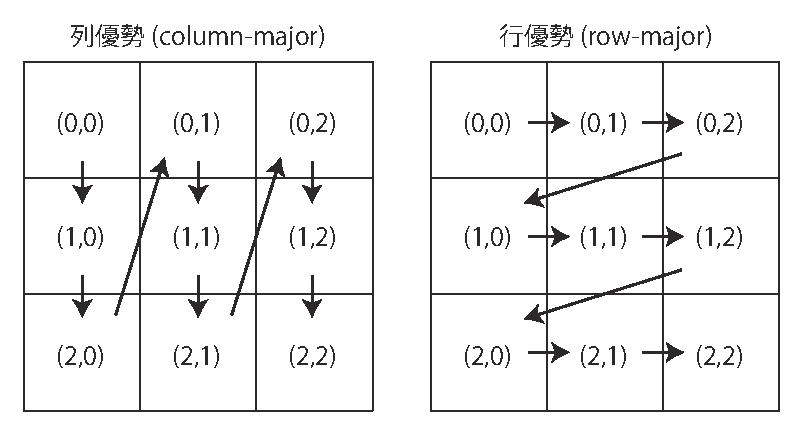
\includegraphics{major.pdf}}
\end{figure}
C言語上で行列の\((i,j)\)成分を \texttt{A[i][j]} に代入したもの(row-major)をLAPACKライブラリに渡すと、LAPACK側では要素がcolumn-majorで並んでいると解釈して計算を行う。すなわち、入力行列が転置されてしまう。また、計算結果もC言語から見ると転置された状態で返されることになってしまう。

これを防ぐには、行列の\((i,j)\)成分を \texttt{A[i][j]} ではなく \texttt{A[j][i]} に格納するように決めてプログラムを書けばよいのだが、「常に順番を逆に書く」というのはプログラム作成時に混乱してしまう恐れがある。一つの解決方法は、Cプリプロセッサのマクロ機能を使い、ソースコードの先頭で
\begin{quote}
    \begin{verbatim}
#define mat_elem(mat, i, j) (mat)[(j)][(i)]
\end{verbatim}
\end{quote}
のように \texttt{mat\_elem} 関数を定義することである\footnote{一般的にCプロセッサのマクロの多用は勧められていないが、背に腹は代えられない。}。これにより、プログラム中で行列の\((i,j)\)成分を \texttt{mat\_elem(A, i, j)} と書けるようになる。
\begin{reidai}\label{ex:malloc-2dim-column-major}
    \begin{verbatim}
#include <stdio.h>
#include <stdlib.h>

#define mat_elem(mat, i, j) (mat)[(j)][(i)]

int main(void) {
    const int m = 3;
    const int n = 4;
    double** matrix = (double**)malloc(sizeof(double*) * n);
    if (matrix == NULL) {
        printf("Can't allocate memory.\n");
        exit(1);
    }
    matrix[0] = (double*)malloc(sizeof(double) * m * n);
    if (matrix[0] == NULL) {
        printf("Can't allocate memory.\n");
        exit(1);
    }
    for (int i = 1; i < n; ++i) {
        matrix[i] = matrix[i - 1] + m;
    }
    for (int i = 0; i < m; ++i) {
        for (int j = 0; j < n; ++j) {
            mat_elem(matrix, i, j) = (i + 1) * (j + 1);
        }
    }
    for (int i = 0; i < m; ++i) {
        for (int j = 0; j < n; ++j) {
            printf("matrix[%d][%d] = %lf\n", i, j, mat_elem(matrix, i, j));
        }
    }
    free(matrix[0]);
    free(matrix);
    return 0;
}
\end{verbatim}
\end{reidai} \noindent
プログラムの前半で、\(3 \times 4\)ではなく\(4 \times 3\)の2次元配列として行列を作成していることに注意せよ\footnote{列優勢(column-major)の2次元配列の確保や解放のための関数、および要素へのアクセス用のマクロ一式をまとめたものが、\hypertarget{cmatrix}{\texttt{cmatrix.h}} として\url{https://github.com/utphys-comp/cmatrix/} で公開されている。}。

\section{\texttt{segmentation fault}が出たら}
コンパイルは出来たのに、実行してみたら\texttt{segmentation fault}と出てプログラムが強制終了することがある\footnote{``することがある''というのが重要。プログラム自体が全く同じでも異常終了したりしなかったりする。}。こういった場合の典型的な原因と対処法を説明する。

\subsection*{スタックの枯渇}
\ref{ex:array1d}で説明したとおり、動的でない配列を大量に確保するとクラッシュすることがある。他にも関数の呼び出し過多(主に再帰)でも同様の現象が起こることがある。

\clangpara{対処法}
動的配列に変更する。再帰を\texttt{for}などのより簡単な処理に置き換える。

\subsection*{範囲外参照}
動的かそうでないかに関わらず、小さすぎる/大きすぎる値を\texttt{[]}に入れて配列を参照するとクラッシュすることがある。\texttt{malloc}の容量設定ミス(要素数ではなくバイト数)や\texttt{argc}の確認不備でよく発生する。

\clangpara{対処法}
ソースコードを見直す。(例えば1次元配列\texttt{a[N]}に対して参照可能な領域は\texttt{a[0], a[1]..., a[N-1]}だけである。)

\subsection*{ダングリングポインタの参照}
代入を行っていないポインタや\texttt{NULL}ポインタ、すでに解放済みの動的配列にアクセスするとクラッシュすることがある。\texttt{fopen}や\texttt{malloc}でよく発生する。

\clangpara{対処法}
ポインタにアクセスする前に、そのポインタがきちんと有効な対象を指しているかを確認する。\texttt{NULL}チェックを行う。

\section{外部ヘッダの利用}
ここでは、他の誰かが作成してくれたものを如何にして自分のプログラムに組み込むか、ということについて説明する。やや難しい内容であるので、読み飛ばしても構わない。

\subsection{外部ヘッダの利用}
既に何度か出てきているが、\texttt{.h}で終わるファイルをヘッダという。
ヘッダの役割の一つとして関数の宣言や定義\footnote{定義を書く場合にはやや特殊な工夫が必要になるので、自作する場合には気をつけよ。}を書くというものがある。
今回は先程出てきた\hyperlink{cmatrix}{\texttt{cmatrix.h}}を例として、外部ヘッダに書かれた関数の使用方法を説明する。

\url{https://github.com/utphys-comp/cmatrix/}から\texttt{cmatrix.h}をダウンロードしてきて、以下の例\ref{ex:ext_header}と\textbf{同じディレクトリ}に配置しよう。

\begin{reidai}\label{ex:ext_header}
    \begin{verbatim}
#include "cmatrix.h"
#include <stdio.h>

int main(void) {
    const int N = 3;
    double** a = alloc_dmatrix(N, N);
    for (int j = 0; j < N; ++j) {
        for (int i = 0; i < N; ++i) {
            mat_elem(a, i, j) = i + j * N;
        }
    }
    fprint_dmatrix(stdout, N, N, a);
    free_dmatrix(a);
    return 0;
}
\end{verbatim}
\end{reidai}
ここで新しく出てきた\texttt{\#include "file"}の記法はただ通常の\texttt{\#include <file>}とヘッダ検索の順序が異なるだけのものである。

コンパイルにはいつもどおりでよい。

\begin{commandline2}
    \prompt \underline{gcc \ref{ex:ext_header}c -Wall -Wextra}
\end{commandline2} \noindent

\clangpara{コンパイラにヘッダの場所を教える}
先程は\texttt{.c}と同じ場所に\texttt{.h}を置いたので、特に何もせずともコンパイルができた。しかし実際にはもっと込み入った場所に置く必要が出てくる場合もある。
そんなときには以下の方法を試してみよう。
\begin{description}
    \item[明示的に場所を指定する]\mbox{}\\
          \texttt{gcc}に\texttt{-I}オプションを与えると、指定したディレクトリをヘッダのある場所として検索しに行くようになる。
    \item[\texttt{CPATH}を設定する]\mbox{}\\
          詳しく説明はしないが、\texttt{export}コマンドを使って\texttt{CPATH}という環境変数を改変することで\texttt{gcc}がヘッダを探索しに行く場所を増やすことができる。変更はターミナルからログアウトするまでずっと有効である。
    \item[シンボリックリンクを貼る]\mbox{}\\
          \texttt{ln -s}を使ってシンボリックリンクを作ると、全く別の場所にあるヘッダがあたかも\texttt{.c}の隣に置いてあるかのように偽装することができる。参照先のファイルを変更すると手元にあるリンクも自動でそれに追従するので、コピーするよりもスマートである。
\end{description}

\subsection{外部ライブラリの利用}
次は同じようなことをライブラリに対してやってみよう。例として何度か出てきているLAPACKを使用する。標準的な環境では特に何もせずとも使えるはずであるが、以下のサンプルが動かないようなら自分の環境に合わせた方法でインストールすること。

以下の例\ref{ex:ext_lib}を\texttt{cmatrix.h}と同じディレクトリに配置しよう。

\begin{reidai}\label{ex:ext_lib}
    \begin{verbatim}
#include "cmatrix.h"
#include <assert.h>
#include <stdio.h>

extern void dgesv_(const int*, const int*, double*, const int*, int*, double*,
    const int*, int*);

int main(void) {
    const int N = 3;
    const int NRHS = 1;
    const int LDA = N;
    const int LDB = N;
    double** a = alloc_dmatrix(N, N);
    double* b = alloc_dvector(N);
    int* ipiv = alloc_ivector(N);
    for (int i = 0; i < N; ++i) {
        mat_elem(a, i, i) = 1;
        if (i + 1 != N) {
            mat_elem(a, i, i + 1) = -1;
        }
    }
    b[N - 1] = 1;
    int info;
    dgesv_(&N, &NRHS, mat_ptr(a), &LDA, vec_ptr(ipiv), vec_ptr(b), &LDB, &info);
    assert(info == 0);
    fprint_dvector(stdout, N, b);
    free_dmatrix(a);
    free_dvector(b);
    free_ivector(ipiv);
    return 0;
}
\end{verbatim}
\end{reidai}
今回は\texttt{-llapack -lblas}のオプションが必要になる。LAPACKがBLASに依存している都合上、\texttt{-l}の順番を変えてはならない。

\begin{commandline2}
    \prompt \underline{gcc \ref{ex:ext_lib}c -llapack -lblas -Wall -Wextra}
\end{commandline2} \noindent

ここで何をしているのかについては説明しないが、\url{https://netlib.org/lapack/explore-html/index.html}を使えば調べられる。
最初に書いてある\texttt{dgesv\_}の宣言部分は\ref{ex:fort}でやっていることと本質的に同じであるが、LAPACKのソースを見て引数の型を調べるのは大変なので、そのときにもこのページが役に立つだろう\footnote{安全性のためFortranにおける入力専用変数にはすべて\texttt{const}をつけてみたが、難しかったら取り除いても構わない。}。

\clangpara{コンパイラにライブラリの場所を教える}
今回何も工夫をせずともコンパイルができたのは、LAPACKがシステムの奥深くに配置されており、その場所が\texttt{gcc}の自動探索対象箇所であったからである\footnote{インストールの方法によってはそういった場所に置いてくれないこともある。}。よってこれほどすんなりとは行かないことも十分ありえる。
そんなときには以下の方法を試してみよう。
\begin{description}
    \item[明示的に場所を指定する]\mbox{}\\
          \texttt{gcc}に\texttt{-L}オプションを与えると、指定したディレクトリをライブラリのある場所として探索しに行くようになる。
    \item[\texttt{LD\_LIBRARY\_PATH}を設定する]\mbox{}\\
          詳しく説明はしないが、\texttt{export}コマンドを使って\texttt{LD\_LIBRARY\_PATH}という環境変数を改変することで\texttt{gcc}がライブラリを探索しに行く場所を増やすことができる。変更はターミナルからログアウトするまでずっと有効である。
\end{description}

\section{外部ツールの利用}
C言語でのプログラミングにおいて有用な外部ツールをいくつか紹介する。あくまで``紹介''に留めるので、使い方は各自調べること。
\begin{description}
    \item[make]\mbox{}\\
          コンパイル用コマンドを管理するツール。
    \item[cmake]\mbox{}\\
          コンパイルの設定、依存関係、テストなどを管理するツール。
    \item[git]\mbox{}\\
          変更履歴を管理するツール。
    \item[gdb]\mbox{}\\
          デバッガ。指定した行で処理を止めたり、変数の中身を覗いたり書き換えたりできる。
    \item[valgrind]\mbox{}\\
          メモリリークや範囲外参照を検出できるツール。
    \item[プロファイラ]\mbox{}\\
          プログラムの処理に時間を要している部分を解析するツール。gprofやvtuneなどが有名。
    \item[フォーマッタ]\mbox{}\\
          インデントやスペース等を全自動で揃えてくれるツール。C用としてはclang-formatが有名。
\end{description}

\section{練習問題の解答例}

以下に練習問題の解答例を示す。さまざまなプログラムの書き方があるので、これらの解答例にこだわらないこと。全く分からない場合に参考にする程度が望ましい。
\begin{renshuu-answer}{prob:2-1}
\baselineskip=12pt
\begin{verbatim}
#include <stdio.h>

int main(void) {
    /* ax+b=0 */
    const double a = 4.0;
    const double b = 1.0;
    printf("ax+b=0\n");
    printf("  a = %lf\n", a);
    printf("  b = %lf\n\n", b);
    if (a == 0.0) {
        if (b == 0.0) {
            printf("  x = all\n");
        } else {
            printf("  x = nothing\n");
        }
    } else {
        printf("  x = %lf\n", -b / a);
    }
    return 0;
}
\end{verbatim}
\end{renshuu-answer}
\begin{renshuu-answer}{prob:2-2}
\baselineskip=12pt
\begin{verbatim}
#include <stdio.h>
#include <stdlib.h>

int main(void) {
    /* calculate "n!" */
    const int n = 10;
    if (n < 0) {
        printf("Can't calculate n!.\n");
        printf("n = %d\n", n);
        exit(1);
    }
    int ans = 1;
    for (int i = 1; i <= n; ++i) {
        ans *= i;
    }
    printf("%d! = %d\n", n, ans);
    return 0;
}
\end{verbatim}
\end{renshuu-answer}
\begin{renshuu-answer}{prob:2-3}
\baselineskip=12pt
\begin{verbatim}
#include <stdio.h>

int main(void) {
    /* n madeno sosuu. */
    const int n = 100;
    printf("%d madeno sosuu = ", n);
    int ans = 2;
    while (ans <= n) {
        int flag = 1;
        for (int i = 2; i < ans; ++i) {
            if (ans % i == 0) {
                flag = 0;
                break;
            }
        }
        if (flag == 1) {
            printf("%d, ", ans);
        }
        ++ans;
    }
    printf("\n");
    return 0;
}
\end{verbatim}
\end{renshuu-answer}
\begin{renshuu-answer}{prob:3-1}
\baselineskip=12pt
\begin{verbatim}
#include <stdio.h>

int main(void) {
    int a[5] = { 1, 2, 3, 4, 5 };
    for (int i = 0; i < 5; ++i) {
        printf("Start: a[%d] = %d\n", i, a[i]);
    }
    int b[5];
    for (int i = 0; i < 5; ++i) {
        b[i] = a[i];
        a[i] = 0;
        printf("End  : a[%d] = %d, b[%d] = %d\n", i, a[i], i, b[i]);
    }
    return 0;
}
\end{verbatim}
\end{renshuu-answer}
\begin{renshuu-answer}{prob:3-2}
\baselineskip=12pt
\begin{verbatim}
#include <stdio.h>

void seki(double a[2][2], double b[2][2], double c[2][2]) {
    c[0][0] = a[0][0] * b[0][0] + a[0][1] * b[1][0];
    c[0][1] = a[0][0] * b[0][1] + a[0][1] * b[1][1];
    c[1][0] = a[1][0] * b[0][0] + a[1][1] * b[1][0];
    c[1][1] = a[1][0] * b[0][1] + a[1][1] * b[1][1];
}

int main(void) {
    double a[2][2] = { { 1.0, 2.0 }, { 3.0, 4.0 } };
    double b[2][2] = { { -1.0, -2.0 }, { -3.0, -4.0 } };
    for (int i = 0; i < 2; ++i) {
        for (int j = 0; j < 2; ++j) {
            printf("a[%d][%d] = %lf, b[%d][%d] = %lf\n", i, j, a[i][j], i, j,
                b[i][j]);
        }
    }
    double c[2][2];
    seki(a, b, c);
    for (int i = 0; i < 2; ++i) {
        for (int j = 0; j < 2; ++j) {
            printf("(a x b)[%d][%d] = %lf\n", i, j, c[i][j]);
        }
    }
    return 0;
}
\end{verbatim}
\end{renshuu-answer}
\begin{renshuu-answer}{prob:4-1}
\baselineskip=12pt
\begin{verbatim}
#include <stdio.h>
#include <stdlib.h>
#include <string.h>

int main(void) {
    /* calculate "n!" */
    int n;
    printf("Input(int): ");
    scanf("%d", &n);
    if (n < 0) {
        printf("Can't calculate n!.\n");
        printf("n = %d\n", n);
        exit(1);
    }
    int ans = 1;
    for (int i = 1; i <= n; ++i) {
        ans *= i;
    }
    printf("%d! = %d\n", n, ans);
    return 0;
}
\end{verbatim}
\end{renshuu-answer}
\begin{renshuu-answer}{prob:5-1}
\baselineskip=12pt
\begin{verbatim}
#include <stdio.h>

int main(void) {
    int array[10];
    int* p;
    for (int i = 0; i < 10; ++i) {
        array[i] = i * i;
    }
    for (int i = 0; i < 10; ++i) {
        printf("array[%d] = %d\n", i, *(array + i));
    }
    for (int i = 0; i < 10; ++i) {
        p = &(array[i]);
        printf("array[%d] = %d\n", i, *p);
    }
    return 0;
}
\end{verbatim}
\end{renshuu-answer}
\begin{renshuu-answer}{prob:7-1}
\baselineskip=12pt
\begin{verbatim}
#include <stdio.h>

struct date {
    unsigned day, month;
    unsigned days;
};

int main(void) {
    const unsigned nMonth[12] = { 31, 28, 31, 30, 31, 30, 31, 31, 30, 31, 30,
        31 };
    struct date inputDay;
    printf("Input(month & day) :\n");
    printf("             month :");
    scanf("%d", &(inputDay.month));
    printf("             day   :");
    scanf("%d", &(inputDay.day));
    inputDay.days = 0;
    for (int i = 1; i < inputDay.month; ++i) {
        inputDay.days += nMonth[i - 1];
    }
    inputDay.days += inputDay.day;
    printf("%d/%d = %d days from 1/1\n", inputDay.month, inputDay.day,
        inputDay.days);
    return 0;
}
\end{verbatim}
\end{renshuu-answer}


\input{latex}

\end{document}
